\documentclass{nthu_thesis}
%DIF LATEXDIFF DIFFERENCE FILE
%DIF DEL /tmp/claude-1012/-home-S113065528/a8fe086e-70e3-42ef-84a7-129bcf41ec84/scratchpad/old_thesis/main.tex   Fri Jul 31 10:55:00 2026
%DIF ADD main.tex                                                                                                Thu Jul 23 12:54:06 2026

\geometry{
  a4paper,
  left=3cm,
  right=3cm,
  top=3cm,
  bottom=3cm,
  bindingoffset=0mm,
  headheight=0pt,
  headsep=0pt,
  footskip=18pt
}
\setlength{\hoffset}{0pt}
\setlength{\oddsidemargin}{15.5pt}
\setlength{\marginparwidth}{0pt}
\setlength{\marginparsep}{0pt}
%DIF PREAMBLE EXTENSION ADDED BY LATEXDIFF
%DIF UNDERLINE PREAMBLE %DIF PREAMBLE
\RequirePackage[normalem]{ulem} %DIF PREAMBLE
\RequirePackage{color}\definecolor{RED}{rgb}{1,0,0}\definecolor{BLUE}{rgb}{0,0,1} %DIF PREAMBLE
\providecommand{\DIFadd}[1]{{\protect\color{blue}\uwave{#1}}} %DIF PREAMBLE
\providecommand{\DIFdel}[1]{{\protect\color{red}\sout{#1}}} %DIF PREAMBLE
%DIF SAFE PREAMBLE %DIF PREAMBLE
\providecommand{\DIFaddbegin}{} %DIF PREAMBLE
\providecommand{\DIFaddend}{} %DIF PREAMBLE
\providecommand{\DIFdelbegin}{} %DIF PREAMBLE
\providecommand{\DIFdelend}{} %DIF PREAMBLE
\providecommand{\DIFmodbegin}{} %DIF PREAMBLE
\providecommand{\DIFmodend}{} %DIF PREAMBLE
%DIF FLOATSAFE PREAMBLE %DIF PREAMBLE
\providecommand{\DIFaddFL}[1]{\DIFadd{#1}} %DIF PREAMBLE
\providecommand{\DIFdelFL}[1]{\DIFdel{#1}} %DIF PREAMBLE
\providecommand{\DIFaddbeginFL}{} %DIF PREAMBLE
\providecommand{\DIFaddendFL}{} %DIF PREAMBLE
\providecommand{\DIFdelbeginFL}{} %DIF PREAMBLE
\providecommand{\DIFdelendFL}{} %DIF PREAMBLE
%DIF COLORLISTINGS PREAMBLE %DIF PREAMBLE
\RequirePackage{listings} %DIF PREAMBLE
\RequirePackage{color} %DIF PREAMBLE
\lstdefinelanguage{DIFcode}{ %DIF PREAMBLE
%DIF DIFCODE_UNDERLINE %DIF PREAMBLE
  moredelim=[il][\color{red}\sout]{\%DIF\ <\ }, %DIF PREAMBLE
  moredelim=[il][\color{blue}\uwave]{\%DIF\ >\ } %DIF PREAMBLE
} %DIF PREAMBLE
\lstdefinestyle{DIFverbatimstyle}{ %DIF PREAMBLE
	language=DIFcode, %DIF PREAMBLE
	basicstyle=\ttfamily, %DIF PREAMBLE
	columns=fullflexible, %DIF PREAMBLE
	keepspaces=true %DIF PREAMBLE
} %DIF PREAMBLE
\lstnewenvironment{DIFverbatim}[1][]{\lstset{style=DIFverbatimstyle}}{} %DIF PREAMBLE
\lstnewenvironment{DIFverbatim*}[1][]{\lstset{style=DIFverbatimstyle,showspaces=true}}{} %DIF PREAMBLE
\lstset{extendedchars=\true,inputencoding=utf8}

%DIF END PREAMBLE EXTENSION ADDED BY LATEXDIFF

\begin{document}
\pagestyle{plain} %This is the default style for most document classes. It places the page number centered in the footer, with an empty header.
\begin{thesiscjk}

\let\cleardoublepage=\clearpage

%%% Necessary fields for this thesis data %%%
% Add your custom class definitions here if any

\newcommand{\degreeZH}{碩}  % 畢業學位，碩 for masters 或 博 for PHD
\newcommand{\degreeEN}{Master's Thesis}  %  Fill in your degree "Master's Thisis" for masters 或 "Doctoral Dissertation" for PHD
\newcommand{\titleZH}{基於自我確信評估與問題拆解的\\自適應知識檢索方法} % 此括弧內填入論文中文標題Chinese title here
\newcommand{\titleEN}{SEEK: Self-certainty Evaluated Evidence-gated Knowledge-retrieval} % 此括弧內填入論文英文標題
\newcommand{\instituteZH}{資訊系統與應用研究所} % 此括弧內填入畢業生所屬學系班
\newcommand{\instituteEN}{Institute of Information Systems and Applications} % Graduation Dept./Inst. Name
\newcommand{\studentID}{113065528} %填入畢業生的學號 your student ID
\newcommand{\studentZH}{簡宏諭} % 此括弧內填入畢業生的中文名字 Graduate's Chinese Name here
\newcommand{\studentEN}{Hung-Yu Chien} %此括弧內填入畢業生的英文姓名 Graduate's Eng. Name here
\newcommand{\advisorZH}{高宏宇} %此括弧內填入指導教授的中文名字，如有兩個，請自行增加
\newcommand{\advisorEN}{Hung-Yu Kao} % 此括弧內填入 advisor's English Name
\newcommand{\yearZH}{115} %此括弧內填入畢業年(民國) Year of ROC  ，就是口試日期的那個月
\newcommand{\monthZH}{7} % Graduation (Oral exam) month of ROC
\newcommand{\yearEN}{2026} % Graduation (oral exam) Year
\newcommand{\monthEN}{July} % Graduation (oral Exam) month


\begin{titlepage}
\newgeometry{a4paper,left=2.54cm,right=3.18cm,top=3.18cm,bottom=2.54cm}  %NTHU cover page setting

 \begin{CJK*}{UTF8}{bkai}
\begin{spacing}{1.3}  
    \begin{center}
       \Huge
        國\hspace{1em}立\hspace{1em}清\hspace{1em}華\hspace{1em}大\hspace{1em}學\\
        National Tsing Hua University\\
        \vspace{1.0 cm}
        \degreeZH~~~士~~~論~~~文\\
        \degreeEN 

    \vspace{2em}  %for controlling veretical space
    \LARGE
        \titleZH\\
        \titleEN \\
    \vspace{2em} %for controlling veretical space

   \Large

%  \setlength\tabcolsep{3pt} % default: 6pt
\renewcommand{\arraystretch}{1.3} % default value is 1.0
      \begin{tabular}{ l }  %l: Left-aligned column.
        系所別：~\instituteZH\\
        Dept.~/~Grad. Inst.:\hspace{0.5em}\instituteEN\\
        學號~ Student ID:\hspace{0.5em}\studentID\\
        研究生~Author：\hspace{0.5em}\studentZH\hspace{0.5em}\studentEN\\
        指導教授~Advisor：\hspace{0.5em}\advisorZH\hspace{0.5em}\advisorEN
    \end{tabular}\\

   \vspace{2em} 

    中~~華~~民~~國~~\zhdigits{\yearZH}~年~~\zhdigits{\monthZH}~月\\
    \monthEN~\yearEN

     \end{center}
\end{spacing}
\end{CJK*}
\end{titlepage}




\restoregeometry  % back to the thesis body geometry after the standard cover

% \cftaddtitleline{toc}{chapter}{學位論文授權書}{}

% 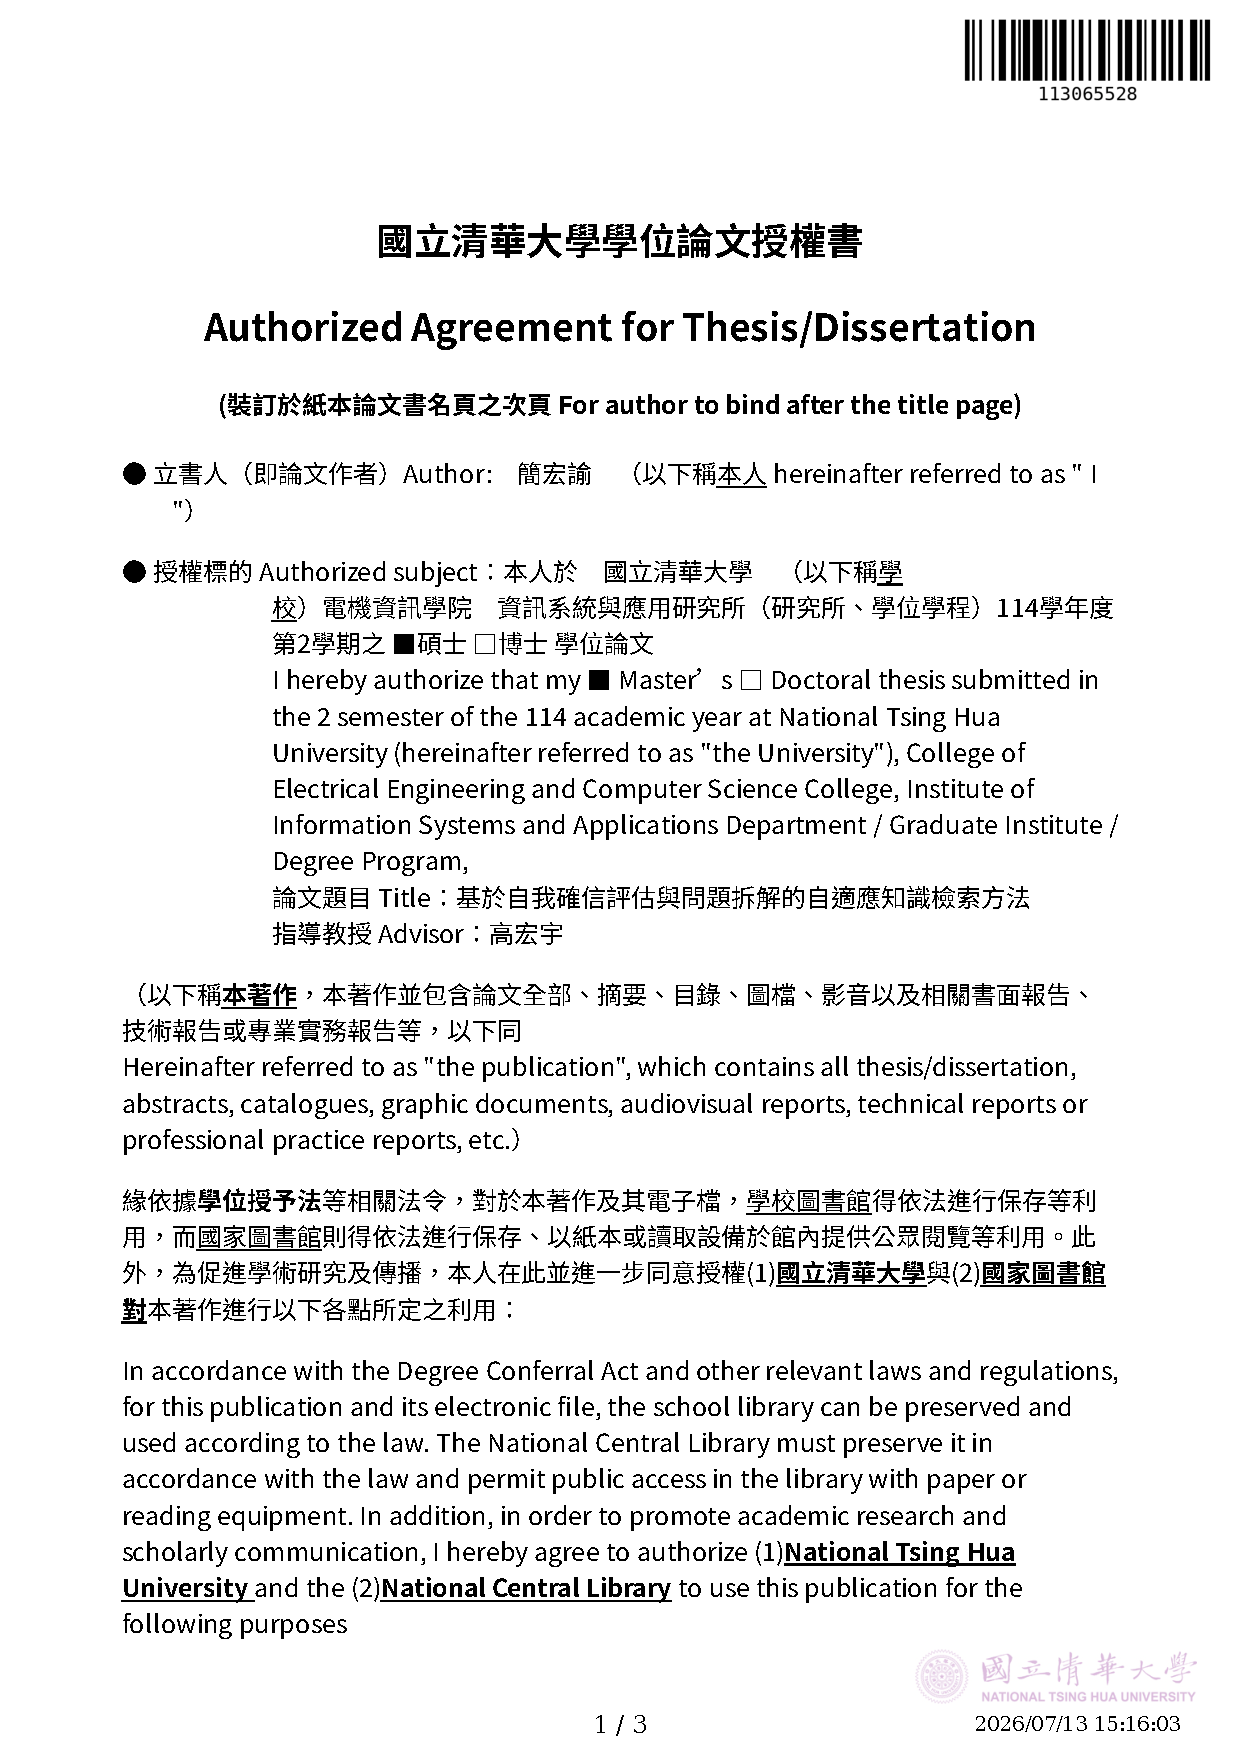
\includepdf[pages=1-3, angle=0, fitpaper=true,
%        keepaspectratio, pagecommand={{\thispagestyle{empty}}},offset=-0.0cm 0.0cm]{./front/Authorized agreement.pdf} %offset=+right +up

% %\cftaddtitleline{<ext>}{<kind>}{<text>}{<page>} intead of using \addcontentsline command  for without page numbering

% \cftaddtitleline{toc}{chapter}{指導教授推薦書}{}

% \includepdf[pages=2, angle=0, fitpaper=true,
%     keepaspectratio, pagecommand={{\thispagestyle{empty}}}]{./front/Advisor Approval Form.pdf}

% \cftaddtitleline{toc}{chapter}{考試委員審定書}{}

% 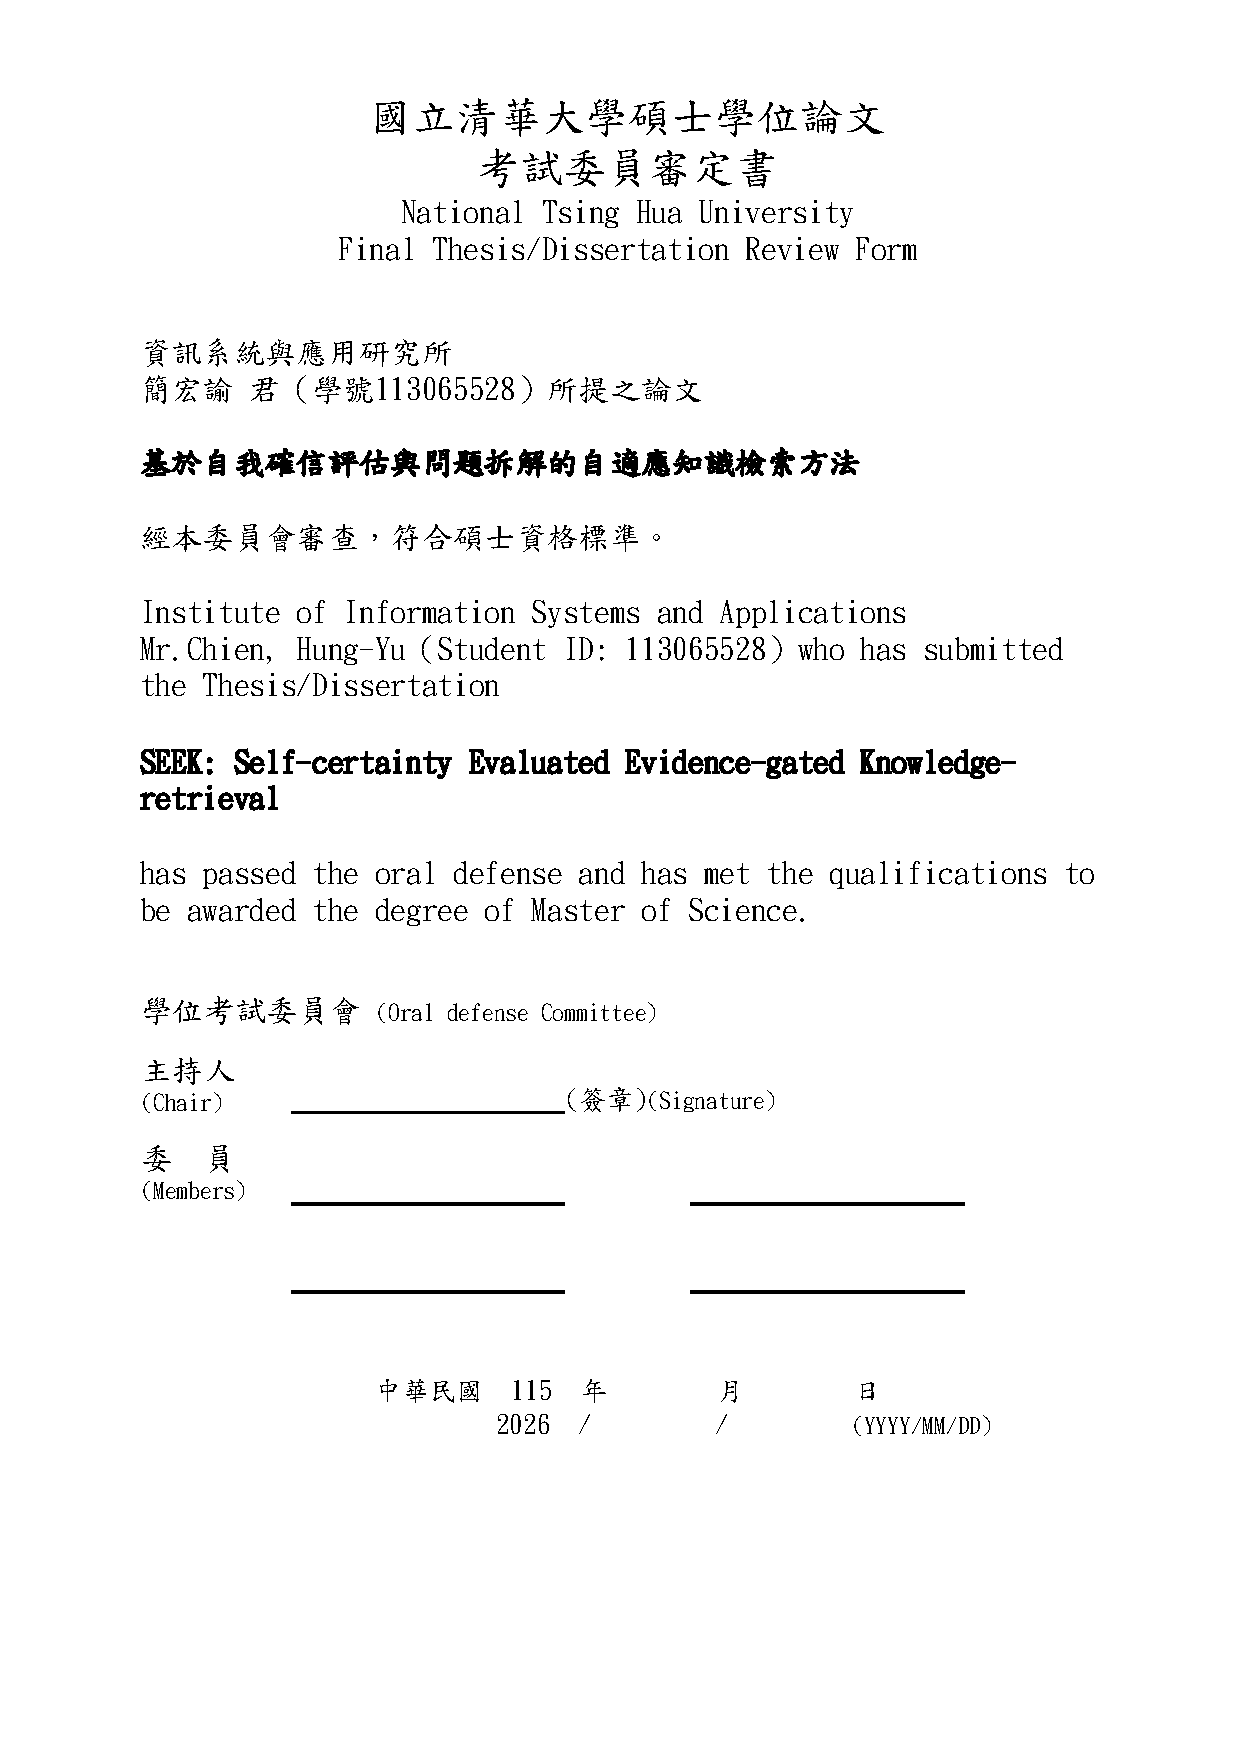
\includepdf[pages=1, angle=0, fitpaper=true,
%        keepaspectratio, pagecommand={{\thispagestyle{empty}}},offset=-0.0cm 0.0cm]{./front/Thesis Review Form.pdf} % offset=+right +up

\frontmatter %Use for book class 

%\pagenumbering{roman} %set lowercase Roman numerals for page numbers if set report class

%%% Necessary 中文摘要%%%

\chapter*{Abstract}
\addcontentsline{toc}{chapter}{Abstract}
This thesis proposes SEEK (Self-certainty Evaluated Evidence-gated Knowledge-retrieval), a lightweight adaptive Retrieval-Augmented Generation (RAG) framework for open-domain question answering. Fixed retrieval can distract simple questions and miss intermediate entities needed by multi-hop questions. Adaptive RAG must decide both whether to retrieve and whether decomposition can expose evidence without discarding global context. Existing approaches rely on coarse routing, imperfect uncertainty signals, or costly learned policies.

SEEK couples step-level retrieval gating with late path selection. A compact decomposer receives one LoRA supervised fine-tuning pass on 12,000 examples from MuSiQue, 2WikiMultihopQA, and PopQA. At inference, SEEK retains direct and decomposed candidates, gates sub-question retrieval with tail-leakage surprisal, adds original-question evidence to decomposed contexts, and uses a training-free type-aware verifier. Decomposition thus remains reversible and routing inspectable.

Across four question-answering datasets under full-corpus Wikipedia retrieval, decomposition improves answer-containing retrieval on the three multi-hop datasets by 5.53--28.03 hit@5 points and leaves single-hop PopQA nearly unchanged at $-0.10$ points. The two answer paths solve different questions, leaving 2.9--6.0 EM of oracle routing headroom. At the accuracy-first threshold of 0.002305, the gate retrieves for 93.84\% of decomposed steps and matches the rounded macro EM of always retrieving while avoiding 6.16\% of retrieval calls. Tail-leakage surprisal is nevertheless not a correctness guarantee, and retrieval gaps account for 47.6--70.1 percent of decomposition-path errors on the multi-hop datasets. Overall, SEEK reaches 41.88 EM and 48.90 F1 on average, compared with 38.45 EM and 45.75 F1 for DeepRAG. The analysis identifies retrieval coverage, bridge-answer propagation, and path selection as the main remaining bottlenecks.

\bigskip
\noindent\textbf{Keywords:} Retrieval-Augmented Generation, Adaptive Retrieval, Multi-hop Question Answering, Tail-Leakage Surprisal, Verifier Routing, Large Language Models
     % Insert English Abstract
\setcounter{page}{1}  %set page begins with i
\clearpage

\chapter*{摘要}
\addcontentsline{toc}{chapter}{摘要}
本論文提出 SEEK (Self-certainty Evaluated Evidence-gated Knowledge-retrieval)，一個用於開放領域問答的輕量化自適應檢索增強生成 (Retrieval-Augmented Generation, RAG) 框架。固定的檢索策略可能為簡單問題引入干擾證據，卻又無法替多跳問題找出後續檢索所需的中介實體。因此，自適應 RAG 不只需要判斷是否檢索，也需要判斷問題分解能否揭露缺失的證據，或反而遺失原始問題中的全域資訊。既有方法多採用粗略的問題層級決策、不完全可靠的詞元層級不確定性訊號，或透過軌跡建構與偏好最佳化學習成本較高的逐步決策策略。

SEEK 將自適應決策分成兩個相互關聯的層次：每個分解子問題是否需要檢索，以及最終答案應取自原始問題路徑或分解路徑。系統以 MuSiQue、2Wiki\-MultihopQA 與 PopQA 的一萬兩千筆資料，透過單次 LoRA 監督式微調訓練一個輕量分解器。推論時，SEEK 同時保留兩條作答路徑，以尾端洩漏驚異度控制子問題檢索，將原始問題的檢索證據加入各分解步驟的上下文，最後再由無需額外訓練、包含答案類型規則的驗證器選出答案。此設計使問題分解成為可撤回的候選策略，並讓路由決策保持可檢視性。

在 HotpotQA、2Wiki\-MultihopQA、MuSiQue 與 PopQA 的完整維基百科語料檢索實驗中，問題分解使三個多跳資料集的答案命中率提升 5.53 至 28.03 個 hit@5 百分點，而單跳 PopQA 僅降低 0.10 個百分點。直接路徑與分解路徑能解決不同問題，理想路由仍有 2.9 至 6.0 EM 的提升空間。在 accuracy-first 閾值 0.002305 下，信心閘門會在 93.84\% 的分解步驟觸發檢索；相較全部檢索，它在論文所報精度下維持相同的平均 EM，同時省下 6.16\% 的檢索呼叫。然而，尾端洩漏驚異度不能保證答案正確，且三個多跳資料集中，47.6\% 至 70.1\% 的分解路徑錯誤源自檢索缺口。整體而言，SEEK 平均達到 41.88 EM 與 48.90 F1，相較之下 DeepRAG 為 38.45 EM 與 45.75 F1；進一步分析則指出，檢索覆蓋、中介答案傳遞與路徑選擇仍是主要瓶頸。

\bigskip
\noindent\textbf{關鍵字：}檢索增強生成、自適應檢索、多跳問答、尾端洩漏驚異度、驗證器路由、大型語言模型
    % 插入中文摘要於此 Insert Chinese Abstract

\clearpage


% \chapter*{Acknowledgements}
% \addcontentsline{toc}{chapter}{Acknowledgements}
% % 致謝 Acknowledgements — 請於此處填寫致謝內容。
% 建議感謝對象包括：指導教授、口試委員、實驗室同仁
% (Intelligent Knowledge Management Lab)、提供研究資源的單位、家人與朋友等。

I would like to express my sincere gratitude to my advisor for the guidance and support throughout this research. I also thank the members of the Intelligent Knowledge Management Lab at National Tsing Hua University, the thesis oral examination committee, and all those who provided computational resources and helpful discussions. Finally, I thank my family and friends for their continuous encouragement.
      % Acknowledgement
% \clearpage

% generate Contents of Tables, lists of figures, tables, 

\tableofcontents
\addcontentsline{toc}{chapter}{Contents}
\clearpage

\listoffigures  % Insert list of figures
\addcontentsline{toc}{chapter}{List of Figures}
\clearpage

\listoftables  % Insert list of tables
\addcontentsline{toc}{chapter}{List of Tables}
\clearpage

%Nomenclature (optional). List unfamiliar terms, symbols, acronyms and their meanings.
%% List of Abbreviations — 縮寫對照表
% 使用 \nomenclature{縮寫}{全名} 新增條目，編譯後會自動排序列出。

\nomenclature{RAG}{Retrieval-Augmented Generation}
\nomenclature{SEEK}{Self-certainty Evaluated Entropy-gated Knowledge-retrieval}
\nomenclature{LLM}{Large Language Model}
\nomenclature{LM}{Language Model}
\nomenclature{QA}{Question Answering}
\nomenclature{SFT}{Supervised Fine-Tuning}
\nomenclature{DPO}{Direct Preference Optimization}
\nomenclature{MDP}{Markov Decision Process}
\nomenclature{EM}{Exact Match}
\nomenclature{AUROC}{Area Under the Receiver Operating Characteristic Curve}
\nomenclature{PPL}{Perplexity}
\nomenclature{CoT}{Chain-of-Thought}
\nomenclature{FLARE}{Forward-Looking Active REtrieval augmented generation}
\nomenclature{NTHU}{National Tsing Hua University}

\renewcommand{\nomname}{List of Abbreviations}
\printnomenclature
    % if needed Nomenclature
%\addcontentsline{toc}{chapter}{Nomenclature}
%\clearpage

% Contents of Thesis

\mainmatter  %for book class only
%\pagenumbering{arabic} % already default for book class, Arabic/Indic page numbers, needed for article class

\pagestyle{plain} %This is the default style for most document classes. It places the page number centered in the footer, with an empty header.
\chapter{Introduction}
\label{ch:introduction}

\section{Background and Motivation}

Large language models (LLMs) have become strong general-purpose generators, but the knowledge encoded in their parameters is necessarily incomplete and fixed at training time. When a question concerns recent events, long-tail entities, or information outside the training distribution, an LLM may still produce a fluent answer even when the underlying facts are unsupported. This behaviour limits the reliability of LLMs in knowledge-intensive applications~\cite{hallucination_survey}.

Retrieval-Augmented Generation (RAG) mitigates this problem by retrieving external passages and conditioning generation on the resulting evidence~\cite{rag_survey}. Because the evidence source can be updated independently of the language model, RAG provides a practical way to extend the model's accessible knowledge without repeated model training. A fixed retrieval strategy, however, is not equally suitable for every question. For a simple question that the model can already answer, irrelevant passages can introduce distractors and additional latency. For a complex multi-hop question, one retrieval query based on the original question may fail to expose the intermediate entity needed to locate the next supporting passage~\cite{ren2023,ircot}.

Adaptive RAG addresses this mismatch by changing the retrieval strategy according to the question or the model's state. Existing approaches include question-level complexity and self-knowledge routers~\cite{adaptiverag,skr}, uncertainty-triggered retrieval during generation~\cite{flare,dragin}, and learned policies that decide retrieval actions at individual reasoning steps~\cite{selfrag,deeprag}. These approaches demonstrate that retrieval need is query-dependent, but each has a different limitation. A question-level route is decided before the intermediate reasoning states are known; uncertainty is an imperfect proxy for correctness; and a learned step-level policy can require additional trajectory construction, supervision, or preference optimisation.

Multi-hop question answering introduces a second decision that is closely coupled with retrieval: whether to decompose the question. Question decomposition can convert a compositional question into shorter sub-questions that expose bridge entities and form more precise retrieval queries~\cite{decomprc,break_qdmr}. Nevertheless, decomposition is not uniformly reliable. An incorrect intermediate answer can misdirect later queries, while a short sub-question can omit comparison targets, entity pairs, or disambiguating conditions from the original question. Forcing every question through a decomposed path may therefore discard useful global context even when the retrieved passages themselves are relevant.

This thesis consequently frames adaptive RAG as a \emph{decomposition-routing problem}. A system should decide at two levels: whether each decomposed sub-question requires external evidence, and whether the final answer should be taken from the original-question path or the decomposed reasoning path. Preserving both paths makes decomposition a candidate strategy rather than an irreversible early commitment. This perspective motivates SEEK (Self-certainty Evaluated Evidence-gated Knowledge-retrieval), a lightweight framework that trains a compact decomposer but keeps retrieval gating and final path verification transparent and training-free.

Accordingly, this thesis investigates whether competitive adaptive RAG can be achieved with lightweight decomposition training and interpretable inference-time routing, without learning a separate retrieval policy. Its objectives are to produce structurally reliable and executable sub-questions, examine both the value and the limits of token-level self-certainty for sub-question retrieval, design a context-preserving dual-path procedure with transparent final verification, and evaluate the resulting framework across single-hop and multi-hop open-domain question answering in terms of accuracy, retrieval behaviour, offline adaptation cost, and failure modes.

\section{Research Contributions}

Our contributions are as follows:

\begin{enumerate}
    \item \textbf{Dual-path decomposition routing.} This thesis treats adaptive RAG as a choice between an original-question answer path and a decomposed answer path, rather than only a retrieve-or-skip decision. SEEK keeps both candidates until a final verification step, so decomposition becomes a reversible strategy instead of an early commitment. The two paths prove complementary: in the final traces, an oracle choice between them would add a further 2.9 to 6.0 EM, and the training-free verifier recovers part of this headroom.

    \item \textbf{A low-cost executable decomposer.} The decomposer is adapted in a single supervised LoRA~\cite{lora} pass on 12{,}000 examples and emits KG-style \texttt{entity >> relation} sub-questions with explicit \texttt{\#N} dependencies that resolve into directly executable retrieval queries. Keeping original-question evidence available at every decomposed step preserves global context that short sub-questions may omit, without changing the decomposer or training another retriever.

    \item \textbf{A simple confidence gate with a measured accuracy--retrieval trade-off.} Tail-leakage surprisal, computed from the probability mass the model keeps within its own top-five token candidates during a single greedy pass, gates sub-question retrieval. \DIFaddbegin \DIFadd{The signal is motivated by a R\'enyi-entropy probe and an exact decomposition of token entropy, which together show that what predicts answer errors is the total probability mass leaking past the model's leading candidates, rather than competition among those candidates or the arrangement of the leaked mass within the tail. }\DIFaddend At the accuracy-first threshold, the gate retrieves for 93.84\% of decomposed steps and matches the rounded macro EM of always retrieving while avoiding 6.16\% of retrieval calls.

    \item \textbf{Training-free late verification.} A deterministic verifier reads direct-answer confidence, decomposition stability, and answer-type compatibility, and selects the final path so that every routing decision remains inspectable. The oracle comparison quantifies the remaining selection headroom without attributing candidate-generation gains to the verifier itself.
\end{enumerate}

\chapter{Related Work}
\label{ch:related}

\section{Adaptive RAG}
\label{sec:adaptive-rag}

Retrieval-Augmented Generation (RAG)~\cite{rag_survey} augments a parametric language model with a non-parametric retriever, allowing the model to condition its generation on external evidence rather than relying only on parameters learned during pretraining. A typical RAG pipeline can be described as five stages~\cite{ragtext_survey}:

\begin{enumerate}
    \item \textbf{Indexing.} The source corpus is segmented into passages, and each passage is stored in a form that supports retrieval, such as sparse lexical indexes or dense vector representations.
    \item \textbf{Query manipulation.} The input question may be rewritten, expanded, normalised, or decomposed so that the retriever can better match it with relevant evidence.
    \item \textbf{Retrieval.} The system selects candidate passages from the indexed corpus, \mbox{commonly} using sparse lexical matching, dense vector similarity, or a hybrid retrieval strategy.
    \item \textbf{Post-retrieval processing.} The initially retrieved passages may be filtered, reranked, compressed, or otherwise refined before they are passed to the generator.
    \item \textbf{Generation.} The language model conditions on the selected evidence and produces the final answer, ideally grounding its output in the retrieved passages.
\end{enumerate}

This retrieve-then-generate paradigm is now widely used to make language model outputs more factual in question answering, explanation writing, and other knowledge-intensive tasks. Its central advantage is that factual evidence can be updated externally without retraining the language model. For multi-hop question answering, however, the quality of the retrieved evidence depends strongly on the query that is issued at each step: a single original question may not contain the intermediate entity needed to retrieve the next supporting passage.

This fixed retrieval assumption creates two well-documented failure modes:

\begin{itemize}
    \item \textbf{Noise injection on easy queries.} For questions the model already knows (e.g.\ ``Who wrote \emph{Hamlet}?''), retrieved passages introduce distractor entities that can override correct parametric knowledge~\cite{popqa,ren2023}.
    \item \textbf{Insufficient evidence on hard queries.} For multi-hop questions, a single retrieval pass rarely surfaces all bridging entities, leading to incomplete or compositionally wrong answers~\cite{ircot}.
\end{itemize}

These two failure modes motivate adaptive retrieval: deciding \emph{when} retrieval is \mbox{useful}, \emph{how much} evidence to fetch, and what signal should determine the gate.

Rather than assuming a fixed retrieve-then-read pipeline, adaptive RAG changes the retrieval path according to the input question, the model state, or the current \mbox{reasoning} step. Some methods decide before generation, using a complexity router or a self-knowledge estimate. Others trigger retrieval from uncertainty observed during generation. A third group learns retrieval actions as part of the generation or reasoning policy. These distinctions structure the discussion below.

\paragraph{Question-level routing.}

A first line of work makes the retrieval decision before generation. These systems inspect the input question and route it to a direct-answer path or a retrieval pipeline, often using a trained classifier or a self-knowledge estimate.

\textbf{Adaptive-RAG}~\cite{adaptiverag} routes each incoming query to one of three retrieval strategies according to its predicted complexity. Easy questions are answered without retrieval, medium-complexity questions use a single retrieval step, and complex questions are routed to a multi-step retrieve-and-reason pipeline such as IRCoT~\cite{ircot}. The router is a T5-Large classifier trained with automatically derived labels. Each training question is assigned to the cheapest strategy that still produces the correct answer, so the classifier learns a cost-aware mapping from question complexity to retrieval depth. This design reduces unnecessary retrieval compared with always using a multi-step pipeline, but the route itself remains a coarse question-level decision.

\textbf{SKR}~\cite{skr} approaches adaptive retrieval from the perspective of self-knowledge. Instead of predicting general question complexity, SKR estimates whether the language model is likely to know the answer from its own parametric memory. If the question is judged as known, the model answers directly; if it is judged as unknown, external retrieval is invoked. This judgement can be implemented with a trained classifier or with memory-based self-knowledge strategies. In the classifier setting, SKR is a binary retrieval gate: it decides whether to retrieve, but does not distinguish between single-step and multi-step retrieval. Therefore, compared with Adaptive-RAG, SKR gives a more direct estimate of whether retrieval is needed, but it still commits to a question-level decision before reasoning begins.


\paragraph{Uncertainty-triggered retrieval.}

A second line of work delays the retrieval decision until generation, using uncertainty signals from the model itself. These methods are often training-free, since the retrieval decision is derived from token probabilities, entropy, \mbox{attention} patterns, or internal model states rather than from an additional trained classifier.

\textbf{FLARE}~\cite{flare} moves the retrieval decision from the question level to the generation level. At each step, it first drafts a tentative next sentence and checks whether the sentence contains low-confidence tokens. If the confidence falls below a threshold, the tentative sentence is used to formulate a retrieval query, and the model regenerates the sentence with the retrieved evidence. This design allows retrieval to occur only when the model appears uncertain during generation. However, token probability is only an indirect proxy for factual uncertainty. A low-probability token may reflect lexical variation rather than missing knowledge, and sentence-level regeneration may not align well with multi-hop reasoning, where the natural decision unit is often a sub-question.

\textbf{DRAGIN}~\cite{dragin} further refines dynamic retrieval by considering both when to retrieve and what to retrieve. Its \emph{Real-time Information Needs Detection} (RIND) module estimates whether the current generation state requires external evidence, while its \emph{Query \mbox{Formulation} based on Self-attention} (QFS) module constructs retrieval queries from salient \mbox{context} tokens instead of relying only on the most recent sentence. Compared with FLARE, DRAGIN provides a more context-aware retrieval trigger and query formulation strategy. Nevertheless, its decision is still made at the token-generation level, which can be mismatched with explicit sub-question reasoning, and it introduces additional overhead from attention-based query construction.

\textbf{SeaKR}~\cite{seakr} estimates retrieval need from the model's internal states rather than from output probabilities alone. It activates retrieval when the model exhibits high self-aware uncertainty and reranks retrieved passages according to how much they reduce that uncertainty. This makes the retrieval signal more closely tied to the model's internal generation dynamics than token-level probability alone. However, the signal is still an estimate of \mbox{uncertainty} rather than a direct measure of answer correctness. A model may be uncertain for reasons unrelated to missing external knowledge, and retrieval may not necessarily improve the answer even when uncertainty is high.

\textbf{TARG}~\cite{targ} studies adaptive retrieval as a training-free, single-shot decision. It generates a short no-context draft and computes uncertainty from the prefix logits to decide whether retrieval should be invoked. In addition to entropy, TARG considers a top-1/top-2 logit-margin signal and a small-sample variance signal. Its main strength is that it \mbox{provides} a lightweight retrieval gate without training an auxiliary classifier or modifying the language model. However, TARG makes one gating decision for the whole question, even on multi-hop benchmarks such as MuSiQue. Its behaviour in decomposition-based retrieval settings, where each sub-question may need its own decision, therefore remains less explored.

Across this family, uncertainty provides a useful and interpretable signal for adaptive retrieval, but it remains an imperfect proxy. Low uncertainty does not guarantee a correct answer, and high uncertainty does not always indicate that retrieval will help. SEEK addresses this limitation by using tail-leakage surprisal both as a sub-question retrieval signal and as the confidence component of a late verifier, rather than treating a single uncertainty score as a hard router for the entire question.

\paragraph{Learned retrieval policies.}

A third line of work makes retrieval control part of the model's learned generation or reasoning behaviour, rather than relying on a front-end router or a hand-set uncertainty threshold.

\textbf{Self-RAG}~\cite{selfrag} trains the language model to generate special reflection tokens that control retrieval and evaluate retrieved passages. For example, the model can emit \texttt{[Retrieve]} to decide whether external evidence is needed, and then use additional tokens to judge whether a passage is relevant, supportive, or useful. This design makes retrieval part of generation itself, rather than a separate preprocessing step. However, it requires fine-tuning with reflection-token supervision and a custom decoding procedure that interleaves normal text generation with retrieval-related decisions.

\textbf{DeepRAG}~\cite{deeprag} formulates retrieval-augmented reasoning as a step-by-step decision process. At each sub-query, the model chooses between answering from parametric memory and issuing a retrieval call. Its training procedure first uses binary tree search to explore both choices for each sub-query, and then applies preference-based calibration to refine the retrieval decision at each sub-query. This design gives it strong sub-question-level retrieval control, but the cost is substantial. Tree-search rollout becomes expensive as the number of reasoning steps grows, preference pairs must be carefully constructed, and the final retrieval policy is learned implicitly rather than exposed as an interpretable score.

A related line of work studies retrieval cost more directly. \textbf{Fast-or-Better}~\cite{fastorbetter} trains two complexity classifiers, one prioritising accuracy and the other prioritising retrieval efficiency, and exposes a user-controlled parameter that interpolates between them, so the accuracy--cost trade-off is no longer fixed at a single operating point. This view reinforces an important point for adaptive RAG: retrieval should be evaluated not only by accuracy, but also by the cost required to obtain that accuracy.

SEEK is closest in spirit to DeepRAG because both methods make retrieval decisions at the sub-question level. The key difference is that SEEK avoids tree search and preference optimisation. It uses a single supervised decomposer and replaces the learned retrieval policy with a training-free verifier based on confidence, decomposition stability, answer type, and whether the direct path and the decomposed path give the same answer.

Overall, SEEK occupies the under-explored region of \emph{late verifier-based routing with interpretable, training-free signals}: only a single SFT pass is needed for the decomposer, and the final route is decided by transparent query-level diagnostics rather than a learned policy.

\section{Reasoning and Knowledge Boundaries in RAG}
\label{sec:reasoning-rag}
\label{sec:knowledge-boundary}

A parallel thread focuses on \emph{how} to retrieve and reason once retrieval is deemed necessary, independent of the gate.

The foundational technique is \textbf{IRCoT}~\cite{ircot}, which interleaves chain-of-thought reasoning with retrieval: after each generated CoT sentence, the partial reasoning becomes the next query. IRCoT is the canonical ``multi-step'' retrieve-and-reason implementation, but its retrieval count grows linearly in the CoT length, regardless of whether intermediate steps are factually difficult. Question decomposition provides a complementary way to structure multi-hop QA. Rather than retrieving after each free-form reasoning sentence, decomposition-based methods explicitly split a complex question into simpler sub-questions that can be answered independently or sequentially. Early systems such as \textbf{DecompRC}~\cite{decomprc} show that compositional questions can be reduced to single-hop reading-comprehension steps, while \textbf{BREAK/QDMR}~\cite{break_qdmr} formalises decomposition as an ordered sequence of natural-language operations required to answer the original question. SEEK inherits this decomposition paradigm, but uses it primarily as an inspectable reasoning path: it preserves the original-question context for decomposed steps, evaluates whether the generated sub-questions are useful, and verifies whether the direct or decomposed answer should be trusted.

More recent work synthesises reasoning data to internalise the retrieve-and-reason loop. \textbf{Auto-RAG}~\cite{autorag} autonomously synthesises multi-turn retrieval--reasoning trajectories and fine-tunes on them, so that the model plans its own retrieval steps without hand-crafted prompts. \textbf{Search-o1}~\cite{searcho1} embeds retrieval inside a large reasoning model in an agentic loop, augmenting o1-style long-chain reasoning with on-demand search and a document-reasoning module that distils retrieved passages before they re-enter the chain. \textbf{AirRAG}~\cite{airrag} activates the model's intrinsic reasoning by combining Monte Carlo Tree Search with self-consistency to explore alternative solution paths. These methods substantially strengthen the reasoning side of RAG, but they rely on heavy data synthesis or search-time expansion; SEEK instead keeps the reasoning component a single lightweight SFT decomposer and concentrates its novelty in training-free verification.

Every adaptive method above ultimately rests on a model's ability to recognise its own \emph{knowledge boundary} --- the line between what it reliably knows and what it must look up. A dedicated line of work studies this capacity directly, and we group it into three strands: \emph{self-knowledge elicitation}, \emph{uncertainty estimation}, and the \emph{interaction between the knowledge boundary and retrieval}.

\paragraph{Self-knowledge and its calibration.} A first strand asks whether a model can introspect on what it knows. Kadavath et al.~\cite{kadavath2022} show that LLMs are, to a useful degree, calibrated: a model can be prompted to predict the probability \texttt{P(True)} that its own answer is correct, and these self-judgements correlate with actual accuracy --- though calibration degrades on out-of-distribution questions. Yin et al.~\cite{yin2023} construct a ``SelfAware'' benchmark of answerable and unanswerable questions and find that LLMs only partially ``know what they don't know'': self-knowledge can be elicited but lags well behind human performance. From the supervised side, Kapoor et al.~\cite{kapoor2024} argue that models ``must be taught to know what they don't know'', demonstrating that lightweight calibration-tuning or probing substantially sharpens a model's estimate of its own uncertainty. Yin et al.~\cite{yin2024} formalise the notion of a knowledge boundary itself, proposing to benchmark a model by probing the frontier of its reliable knowledge rather than by aggregate accuracy alone.

\paragraph{Uncertainty estimation as a boundary signal.} A second strand asks how to \emph{measure} the boundary at inference time. Beyond retrieval-specific methods, recent work on LLM uncertainty quantification compares several confidence estimators for answer correctness, including token entropy, maximum softmax probability, margin-based scores, verbalised confidence, and response consistency~\cite{maqa}. These comparisons show that the reliability of each signal varies across tasks and models. This motivates testing whether entropy is sufficient in SEEK's QA setting, or whether a signal focused on the probability mass escaping the top candidates provides a more discriminative retrieval gate.

Semantic entropy further shows why token-level uncertainty can be limited for natural-language answers: different surface forms may express the same meaning, so uncertainty over token sequences does not always correspond to uncertainty over answers. Kuhn et al.~\cite{semanticuncertainty} introduce \emph{semantic entropy}, which clusters multiple sampled answers by meaning before computing entropy, so that paraphrases of one correct answer do not register as uncertainty; Farquhar et al.~\cite{semanticentropy} scale this idea and show that semantic entropy reliably detects confabulations across QA and biography generation. This observation is important for SEEK because exact QA answers often involve aliases, entity variants, and short spans. The same concern shapes SEEK's choice of signal: competition among the top candidates is often alias-level variation, so tail-leakage surprisal counts only the probability mass that leaks out of the candidate set. We nevertheless treat token-level confidence as a cheap diagnostic signal rather than as a correctness guarantee.

\paragraph{The boundary under retrieval.} A third strand studies the boundary specifically in the RAG setting. Ren et al.~\cite{ren2023} show that retrieval augmentation not only injects evidence but also \emph{reshapes} the boundary: relevant passages let a model answer questions it could not before, while irrelevant or distracting passages can push a previously-correct answer over the boundary into error --- precisely the ``noise injection on easy queries'' failure mode of \S\ref{sec:adaptive-rag}. This makes a per-step boundary estimate, rather than a one-shot query-level one, essential when retrieval and reasoning are interleaved.

These three strands form the conceptual foundation of SEEK. The failure modes of \S\ref{sec:adaptive-rag} --- spurious retrieval on easy queries, missing retrieval on hard ones, and confident hallucination under a hard confidence threshold --- are all symptoms of a poorly localised knowledge boundary. Where confidence-based methods read a single uncertainty proxy and policy-based methods bury the boundary inside a learned policy, SEEK makes the boundary inspectable through a late verifier: confidence, decomposition stability, and answer-type compatibility jointly decide whether the direct or decomposed path should be trusted.

\section{Evaluation Datasets}
\label{sec:evaluation-datasets}

The evaluation of adaptive RAG hinges on datasets that span both single-hop and multi-hop complexity. This thesis uses HotpotQA, 2WikiMultihopQA, MuSiQue, and PopQA to cover both multi-hop reasoning and single-hop factual recall.

\paragraph{HotpotQA.}

HotpotQA~\cite{hotpotqa} is the canonical multi-hop QA benchmark, containing 113K Wikipedia-based questions requiring 2-hop reasoning. Each example provides (a) the question, (b) the gold answer, (c) two gold-supporting paragraphs mixed with eight distractor paragraphs (in the \texttt{distractor} setting), and (d) sentence-level supporting facts. Questions fall into two compositional patterns: \emph{bridge} (the answer to sub-question 1 is the subject of sub-question 2) and \emph{comparison} (two entities are compared along a shared attribute). It is a standard evaluation set for adaptive RAG and multi-hop reasoning systems.

\paragraph{2WikiMultihopQA.}

2WikiMultihopQA~\cite{twowiki} constructs 192K multi-hop questions by leveraging Wikidata knowledge-graph paths, ensuring each question requires traversal of an explicit reasoning chain. It includes four question types (comparison, inference, compositional, and bridge-comparison) and provides KG-triple annotations alongside textual evidence. Compared to HotpotQA, 2WikiMultihopQA is constructed so that its questions are hard to answer through reasoning shortcuts, making it a more reliable test of compositional reasoning.

\paragraph{MuSiQue.}

MuSiQue (\textbf{Mu}ltihop questions via \textbf{Si}ngle-hop \textbf{Que}stions)~\cite{musique} addresses two pathologies of earlier datasets: (i) shortcut answers via single-hop reasoning, and (ii) weak distractor selection. MuSiQue is built by composing 2--4 single-hop questions into chains using strict connectivity criteria, yielding 25K questions of 2-hop, 3-hop, and 4-hop varieties. Importantly, MuSiQue provides the \emph{decomposed} sub-questions as supervision, which makes it a natural training source for decomposer models such as the one used in SEEK. Its high distractor difficulty makes it the hardest of the four datasets in this thesis.

\paragraph{PopQA.}

PopQA~\cite{popqa} is a \emph{single-hop} entity-centric QA dataset of 14K questions, each derived from a Wikidata subject--property--object triple. Critically, PopQA tags each entity with its \emph{popularity} (measured by monthly Wikipedia page views), enabling stratified evaluation of factual recall on long-tail entities. Despite being single-hop, PopQA exposes the over-decomposition failure mode of decomposer-based pipelines: trained on multi-hop data, a decomposer may emit two-step plans even when one step suffices, harming both EM and efficiency.

\paragraph{Single-hop open-domain QA.}

For completeness, prior adaptive-RAG papers also evaluate on \textbf{Natural Questions (NQ)}~\cite{nq}, \textbf{TriviaQA}~\cite{triviaqa}, and \textbf{SQuAD}~\cite{squad}. These are single-hop datasets whose answers typically exist in a single evidence paragraph, and they primarily test whether an adaptive method can correctly \emph{skip} retrieval rather than orchestrate it. This thesis uses PopQA as the representative single-hop test set because it stresses factual recall and over-decomposition on entity-centric questions.

\chapter{Methodology}
\label{ch:method}

This chapter presents \textbf{SEEK} (\textbf{S}elf-certainty \textbf{E}valuated \textbf{E}vidence-gated \textbf{K}nowledge-retrieval), a lightweight adaptive RAG framework that treats question decomposition as a routing problem. SEEK runs both a direct path and a decomposition path, preserves original-question evidence inside decomposed steps, and chooses between the candidate answers using a training-free verifier. The design follows the view that adaptive RAG is more than a retrieve-or-skip problem: a question may need to be answered directly, decomposed into sharper retrieval queries, or repaired with original-question context after decomposition.

\section{Overview}
\label{sec:overview}

Given a question $q$ and an open-domain retrieval corpus $\mathcal{P}$, SEEK produces a final answer $\hat{a}$ through two candidate-generation paths followed by a verifier. Figure~\ref{fig:pipeline} shows the overall pipeline:

\begin{enumerate}
    \item \textbf{Direct path.} The answerer directly answers the original question $q$ with BM25 evidence retrieved from $\mathcal{P}$, producing a direct candidate $a^{\mathrm{dir}}$ and a token-level confidence score $\sigma^{\mathrm{dir}}$ over the generated answer span.
    \item \textbf{Decomposition path.} The decomposer $\mathcal{D}_\theta$ maps $q$ to ordered sub-questions $\{s_1, \ldots, s_n\}$. Each sub-question is answered sequentially, with placeholder substitution, confidence probing, conditional retrieval, original-question evidence union, and a final synthesis step that produces $a^{\mathrm{dec}}$.
    \item \textbf{Training-free verifier.} A deterministic verifier compares $a^{\mathrm{dir}}$ and $a^{\mathrm{dec}}$ using direct-answer confidence, decomposition stability, and answer-type compatibility. It returns either $a^{\mathrm{dir}}$ or $a^{\mathrm{dec}}$ as $\hat{a}$.
\end{enumerate}

\begin{figure}[htbp]
    \centering
    \makebox[\linewidth][c]{\includegraphics[width=1.3\linewidth]{Thesis_overflow.pdf}}
    \caption[SEEK Pipeline]{Overview of SEEK. Stage 1 constructs 12K gold decomposition examples from MuSiQue, 2WikiMultihopQA, and PopQA; Stage 2 trains the LoRA decomposer on this corpus; Stage 3 runs dual-path inference, where the direct path answers the original question with retrieved evidence and the decomposition path answers sub-questions sequentially with confidence-gated retrieval and answer propagation, and a training-free verifier selects the final answer.}
    \label{fig:pipeline}
\end{figure}

\section{Problem Formulation}

We study open-domain question answering: given a natural-language question $q$ and a passage corpus $\mathcal{P}$, the system outputs a short answer span $\hat{a}$, which is evaluated against gold answers by exact match and F1. The questions of interest are often multi-hop, so a single retrieval with the original question may not surface all the required evidence. Let $\mathcal{M}_\theta$ be a pretrained language model, $r(q, \mathcal{P}, k)$ a BM25 retriever over an open-domain corpus $\mathcal{P}$, and $\mathcal{D}_\theta(q)$ a decomposer that emits sub-questions. A conventional retrieve-then-read system produces one answer from one path. SEEK instead constructs two candidates. The direct candidate answers the original question with retrieved evidence:

\[
    a^{\mathrm{dir}} = \mathcal{M}_\theta(q, r(q, \mathcal{P}, k)).
\]

The decomposition candidate first maps the question to an ordered list of sub-questions,

\[
    \{s_1, \ldots, s_n\}=\mathcal{D}_\theta(q),
\]

then answers each sub-question $s_i$ in order to obtain $a_i$, and finally synthesises the pairs into an answer span:

\[
    a^{\mathrm{dec}} = \mathrm{Synth}\left(q, \{(s_i, a_i)\}_{i=1}^{n}\right).
\]

Here $\mathrm{Synth}$ is not a string-level merge but a final generation pass of the base model $\mathcal{M}_\theta$: it reads $q$ together with all pairs $(s_i, a_i)$ and generates the final answer span under the prompt rules described in Section~\ref{sec:gate}.

The final decision is a verifier $v$:

\[
    \hat{a}=v\left(q, a^{\mathrm{dir}}, a^{\mathrm{dec}}, z^{\mathrm{dir}}, z^{\mathrm{dec}}\right),
\]

where $z^{\mathrm{dir}}$ and $z^{\mathrm{dec}}$ are inference-time diagnostic signals such as confidence scores, unresolved placeholders, and whether $a^{\mathrm{dir}}$ and $a^{\mathrm{dec}}$ are the same answer after normalisation. The verifier is a transparent rule set designed to approximate the oracle choice between direct and decomposed reasoning.

\section{Sub-Question Decomposer}
\label{sec:decomposer}

The decomposer emits one sub-question per line, prefixed with \texttt{\#}$\langle i \rangle$\texttt{:}. Each sub-question is expressed as a compact knowledge-graph fragment:

\begin{center}
    \texttt{\#}$i$\texttt{: }$\langle$\emph{entity}$\rangle$\texttt{ >> }$\langle$\emph{relation}$\rangle$
\end{center}

When a sub-question depends on an earlier answer, the placeholder \texttt{\#}$j$ refers to the answer of step $j$. For example:

\begin{center}
\begin{tabular}{ll}
    \texttt{\#1: Inception >> director} & $\rightarrow$ $a_1$ = \texttt{Christopher Nolan}\\
    \texttt{\#2: \#1 >> place of birth} & $\rightarrow$ \texttt{Christopher Nolan >> place of birth}
\end{tabular}
\end{center}

At inference, placeholders are resolved sequentially: \texttt{\#1} stands for the answer text of step 1, not its index. Once step 1 returns $a_1$, \texttt{\#1} in $s_2$ is replaced by that answer before retrieval and answering, as shown in the example above. The KG-triple notation is compact, consistent across datasets, and aligned with Wikidata-style supervision in 2WikiMultihopQA and PopQA.

The fixed instruction used to prompt the decomposer is shown in Figure~\ref{fig:decomposer-prompt}.

\begin{figure}[H]
    \centering
    \vspace{-1.2\baselineskip}
    \includegraphics[width=0.82\textwidth,trim=145bp 500bp 107bp 210bp,clip]{prompt_Decomposer.pdf}
    \caption[Decomposer Prompt]{Fixed instruction prompt used by the decomposer.}
    \label{fig:decomposer-prompt}
\end{figure}

The prompt standardises the output format without imposing a fixed decomposition depth. As Table~\ref{tab:decomp-examples} illustrates, the same representation accommodates one-hop fact lookup, bridge reasoning, comparison, and longer compositional chains.

\begin{table}[htbp]
    \centering
    \caption[Decomposition Patterns by Dataset]{Representative decomposition patterns produced by the SEEK decomposer.}
    \label{tab:decomp-examples}

    \setlength{\tabcolsep}{6pt}
    \small
    \begin{tabular}{ l p{4cm} p{6cm} }
        \toprule
        Dataset & Question type & Decomposition \\
        \midrule
        PopQA & 1-hop fact lookup & \texttt{\#1: George Rankin >> occupation} \\
        \addlinespace
        HotpotQA & 2-hop bridge & \texttt{\#1: Film X >> director} \newline \texttt{\#2: \#1 >> nationality} \\
        \addlinespace
        2WikiMultihopQA & comparison & \texttt{\#1: A >> date of birth} \newline \texttt{\#2: B >> date of birth} \\
        \addlinespace
        MuSiQue & compositional chain & \texttt{\#1: X >> capital} \newline \texttt{\#2: \#1 >> mayor} \newline \texttt{\#3: \#2 >> party} \\
        \bottomrule
    \end{tabular}
\end{table}

\paragraph{Training.} Only the decomposer requires training; the answerer, synthesizer, and verifier are training-free. The decomposer is a LoRA~\cite{lora} adapter on Llama-3-8B-Instruct, trained on 12{,}000 examples drawn equally from MuSiQue gold sub-questions, 2WikiMultihopQA evidence-triple conversions, and PopQA one-step triples. Before the PopQA examples were sampled, all 1{,}000 evaluation question IDs were removed; the resulting 4{,}000 PopQA training questions have zero exact overlap with the evaluation questions. The PopQA component teaches the decomposer that a one-step plan is valid. This improves single-hop robustness, but Chapter~\ref{ch:results} shows that it also creates negative transfer on some multi-hop datasets; the verifier is introduced precisely because no single hard decomposition policy is optimal across all query types. At inference, the adapter is enabled for decomposition and sub-question answering, and disabled for final synthesis, where the base instruction model produces shorter and more stable spans.

\clearpage

\section{Token-Level Confidence Probe}
\label{sec:probe}

The fixed answer-only instruction used for both direct and sub-question answering is shown in Figure~\ref{fig:answer-prompt}.

\begin{figure}[H]
    \centering
    \vspace{-1.2\baselineskip}
    \includegraphics[width=0.82\textwidth,trim=126bp 389bp 126bp 382bp,clip]{prompt_Answer.pdf}
    \caption[Answer Prompt]{Answer-only prompt for direct and sub-question generation.}
    \label{fig:answer-prompt}
\end{figure}

During greedy decoding, SEEK records the softmax distribution $p_t=\mathrm{softmax}(\mathrm{logits}_t)$ for each generated token $t$. All confidence signals in SEEK are derived from these distributions: generation is a single greedy pass, so no resampling-based agreement is available, and no additional model is trained to judge confidence.

\paragraph{Two kinds of uncertainty.} The signal design starts from an observation about how correct and incorrect answers differ at the token level. When the model knows the answer, the probability mass concentrates on a few candidates, and the remaining competition is typically between surface variants of the same answer, such as aliases, casing, or formatting differences. When the model lacks the required knowledge, the mass instead disperses over many unrelated continuations, well beyond any small set of plausible candidates. What separates the two cases is not how evenly the leading candidates split the mass, but whether the mass stays inside a small candidate set at all.

\DIFaddbegin \paragraph{\DIFadd{Locating the signal with R\'enyi entropy.}} \DIFadd{Before committing to a particular functional form, SEEK first asks }\emph{\DIFadd{which region}} \DIFadd{of the next-token distribution carries the error-related information. R\'enyi entropy~\mbox{%DIFAUXCMD
\cite{renyi1961} }\hskip0pt%DIFAUXCMD
offers a controlled instrument for this question, because it leaves the underlying probabilities untouched and changes only the relative emphasis given to high- and low-probability tokens:
}

\begin{equation}
    \DIFadd{H_\alpha(p_t)=\frac{1}{1-\alpha}\log\sum_{v} p_t(v)^{\alpha},
    \qquad \alpha>0,\ \alpha\neq 1,
    \label{eq:renyi}
}\end{equation}

\DIFadd{which recovers Shannon entropy in the limit $\alpha\rightarrow 1$. For $\alpha>1$ the sum is dominated by the largest probabilities, so the measure mainly describes the shape of the head; for $\alpha<1$ small probabilities are amplified, so the measure becomes increasingly sensitive to the tail. This distinction is consequential for LLM next-token distributions: over a vocabulary of more than 128K tokens, the tail consists of tens of thousands of individually negligible probabilities, and Shannon entropy, which weights each token by its own probability, folds their combined effect together with the competition among a handful of leading candidates into a single number. Substituting R\'enyi variants for Shannon entropy inside the same maximum-token-entropy error detector evaluated in Section~\ref{sec:tail-leakage-analysis} isolates the effect of this reweighting while holding everything else fixed; Figure~\ref{fig:renyi-reweight} visualises the reweighting and the resulting detection quality. On the 2WikiMultihopQA direct-path trace, the head-sensitive setting $\alpha=2$ reaches an error-detection AUROC of 0.651, Shannon entropy ($\alpha\rightarrow 1$) reaches 0.671, and the tail-sensitive setting $\alpha=0.5$ improves to 0.716. Detection quality rises monotonically as emphasis moves from the head towards the tail, which is the first piece of evidence that the error-related signal resides in the low-probability region rather than among the leading candidates. R\'enyi entropy nevertheless still compresses the entire distribution into one number: it indicates that the tail matters, but cannot distinguish whether what matters is }\emph{\DIFadd{how much}} \DIFadd{total mass leaks into the tail or }\emph{\DIFadd{how}} \DIFadd{that mass is arranged within it. The remainder of this section separates the two.
}

\begin{figure}[htbp]
    \centering
    \includegraphics[width=\textwidth]{fig_renyi_reweight_auroc.pdf}
    \caption[R\'enyi Reweighting and Error Detection]{\DIFaddFL{R\'enyi reweighting of a next-token distribution and its effect on error detection. Left three panels: the escort distribution $p_t(v)^{\alpha}/\sum_{w} p_t(w)^{\alpha}$ of one fixed next-token distribution under three orders $\alpha$; $\alpha=2$ concentrates emphasis on the head (orange), $\alpha\rightarrow 1$ recovers the Shannon weighting, and $\alpha=0.5$ amplifies the tail (blue). Right: error-detection AUROC of the corresponding maximum-token-entropy detector on the 2WikiMultihopQA direct-path trace rises monotonically as emphasis moves towards the tail.}}
    \label{fig:renyi-reweight}
\end{figure}

\paragraph{\DIFadd{Same entropy, different risk.}} \DIFadd{A minimal example shows why a single entropy value cannot make this separation. Figure~\ref{fig:same-entropy-risk} and Table~\ref{tab:same-entropy-example} construct two next-token distributions for an answer position at which the model chooses between the casing variants }\texttt{\DIFadd{PO}} \DIFadd{and }\texttt{\DIFadd{po}} \DIFadd{of the same answer. The two distributions share identical leading candidates and, by construction, the same Shannon entropy of approximately $1.83$ nats. They differ only in where the remaining probability sits: distribution A retains $0.90$ of its mass inside the five most probable tokens and leaks $10\%$ into a dispersed tail of twelve tokens, whereas distribution B retains only $0.80$ and leaks twice as much mass into a more concentrated tail of five tokens. Entropy cannot separate the two cases because it responds simultaneously to the amount of leaked mass and to how dispersed that mass is: a smaller but more dispersed tail and a larger but more concentrated one sum to the same entropy. For the retrieval decision, however, the relevant event is that twice as much probability has escaped the model's main candidate set, while the competition between the two leading candidates—surface variants of one answer—is benign in both cases. The leakage score introduced below reacts to exactly this difference: $-\log 0.90 = 0.105$ versus $-\log 0.80 = 0.223$, more than doubling where entropy does not move at all.
}

\begin{figure}[htbp]
    \centering
    \includegraphics[width=\textwidth]{fig_same_entropy_risk.pdf}
    \caption[Same Entropy, Different Risk]{\DIFaddFL{The two constructed distributions of Table~\ref{tab:same-entropy-example}. The two leading candidates (orange) are identical and both distributions have a Shannon entropy of $1.83$ nats, yet distribution B leaks twice as much probability mass into the tail (blue). The leakage score $-\log m_t$ more than doubles while entropy does not move.}}
    \label{fig:same-entropy-risk}
\end{figure}

\begin{table}[htbp]
    \centering
    \caption[Same Entropy, Different Risk]{\DIFaddFL{Two constructed next-token distributions with identical leading candidates and equal Shannon entropy (natural logarithm) but different tail mass. The per-token leakage score $-\log m_t$ defined in Section~\ref{sec:probe} separates them, whereas entropy does not.}}
    \label{tab:same-entropy-example}
    \small
    \begin{tabular}{lcc}
        \toprule
         & \DIFaddFL{Distribution A }& \DIFaddFL{Distribution B }\\
        \midrule
        \DIFaddFL{rank 1: }\texttt{\DIFaddFL{PO}} & \DIFaddFL{0.38 }& \DIFaddFL{0.38 }\\
        \DIFaddFL{rank 2: }\texttt{\DIFaddFL{po}} & \DIFaddFL{0.26 }& \DIFaddFL{0.26 }\\
        \DIFaddFL{ranks 3--5 }& \DIFaddFL{0.11 / 0.08 / 0.07 }& \DIFaddFL{0.06 / 0.05 / 0.05 }\\
        \midrule
        \DIFaddFL{top-five retained mass }& \DIFaddFL{0.90 }& \DIFaddFL{0.80 }\\
        \DIFaddFL{tail mass }& \DIFaddFL{0.10 (12 tokens $\times$ 0.83\%) }& \DIFaddFL{0.20 (5 tokens $\times$ 4.0\%) }\\
        \DIFaddFL{Shannon entropy (nats) }& \DIFaddFL{1.83 }& \DIFaddFL{1.83 }\\
        \DIFaddFL{leakage score $-\log m_t$ }& \DIFaddFL{0.105 }& \DIFaddFL{0.223 }\\
        \bottomrule
    \end{tabular}
\end{table}

\DIFaddend \paragraph{Decomposing token entropy.} Token entropy is the usual way to measure this kind of uncertainty, but it mixes the leakage of probability mass out of the candidate set with effects that are unrelated to correctness. Let $V_5(p_t)$ denote the set of the five most probable tokens under $p_t$, and let

\begin{equation}
    m_t = \sum_{v\in V_5(p_t)} p_t(v)
    \label{eq:topk-mass}
\end{equation}

be the probability mass retained within these candidates; the mass $1-m_t$ that leaks into the rest of the vocabulary is the tail. For token entropy $H(p_t)=-\sum_v p_t(v)\log p_t(v)$, the chain rule gives three components:

\begin{equation}
    H(p_t)=H_{\mathrm{B}}(m_t)+m_t\,H(\hat{p}_t^{\,\mathrm{in}})+(1-m_t)\,H(\hat{p}_t^{\,\mathrm{out}}),
    \label{eq:entropy-chain}
\end{equation}

where $H_{\mathrm{B}}$ is the binary entropy of whether the next token falls inside the top five or in the tail, and $\hat{p}_t^{\,\mathrm{in}}$, $\hat{p}_t^{\,\mathrm{out}}$ are the renormalised distributions inside and outside the top-five set. Only the first term reflects whether mass leaks into the tail. The second term measures competition inside the top five, which for correct answers frequently comes from surface variants of the same answer, and the third term describes the composition of the tail, which carries little information about correctness. Mixing the three therefore makes entropy a weaker error signal than the leakage term alone. \DIFaddbegin \DIFadd{This decomposition is an identity, not an approximation: it does not introduce a new uncertainty measure, but makes it possible to test each source of uncertainty separately. Section~\ref{sec:tail-leakage-analysis} performs exactly this test and confirms the reading: scored in isolation over the same traces, the leakage term reaches a macro error-detection AUROC of 0.742, competition inside the top five reaches 0.712, and the composition of the tail reaches 0.502, barely above chance. What predicts errors is how much mass leaves the candidate set, not how the leaked mass is arranged once it has left; this also resolves the ambiguity that the R\'enyi probe left open.
}\DIFaddend 

\paragraph{Tail-leakage surprisal.} The confidence signal of SEEK retains only the top-five mass $m_t$ from this decomposition and transforms it into a monotonic leakage score, while discarding the two within-group entropy terms. Surprisal is the standard information-theoretic measure of how unexpected an event is: an event of probability $p$ carries surprisal $-\log p$. Applying it to the event that generation stays within the candidate set, and accumulating over the answer, gives

\begin{align}
    \mathrm{TL}_t
        &= -\log m_t, \label{eq:tl-token} \\
    \sigma^{\mathrm{tl}}
        &= \sum_{t\in\mathcal{T}} \mathrm{TL}_t
         = -\log \prod_{t\in\mathcal{T}} m_t , \label{eq:tail-leakage}
\end{align}

where $\mathcal{T}$ indexes the generated answer tokens, excluding EOS. $\mathrm{TL}_t$ is the surprisal of staying inside the candidate set at position $t$: it is near zero when the top five candidates retain almost all of the mass, and it grows as mass leaks into the tail.
\DIFaddbegin 

\DIFadd{The transform is deliberately }\emph{\DIFadd{not}} \DIFadd{the binary-entropy term $H_{\mathrm{B}}(m_t)$ of Equation~\eqref{eq:entropy-chain}. A risk score should satisfy a basic monotonicity requirement: the more probability leaves the candidate set, the higher the score, with no reversal at severe leakage. As Figure~\ref{fig:leakage-monotonicity} shows, binary entropy violates this requirement, because as a function of the leaked mass $1-m_t$ it rises, peaks at $1-m_t=0.5$, and then falls again, so a token that leaks most of its mass would receive a score as low as one that leaks almost nothing. The role of the decomposition is therefore to identify $m_t$ as the informative variable, and the role of $-\log m_t$ is to convert that variable into a score that is strictly increasing in the leaked mass and, as a logarithm, additive across positions.
}

\begin{figure}[htbp]
    \centering
    \includegraphics[width=0.92\textwidth]{fig_leakage_monotonicity.pdf}
    \caption[Monotonicity of the Leakage Score]{\DIFaddFL{Binary entropy $H_{\mathrm{B}}(m_t)$ and leakage surprisal $-\log m_t$ as functions of the leaked mass $1-m_t$. Binary entropy peaks at $1-m_t=0.5$ and then falls, so severe leakage would be scored as low as near-certainty, whereas $-\log m_t$ increases strictly with the leaked mass.}}
    \label{fig:leakage-monotonicity}
\end{figure}

\DIFaddend The answer-level score $\sigma^{\mathrm{tl}}$ accumulates this leakage over the generated span. The sum is preferred over a worst-token maximum because a wrong answer often leaks a small amount of mass at several positions rather than a large amount at one, and a maximum-based aggregate cannot accumulate this pattern. \DIFaddbegin \DIFadd{As a direct check that the score orders risk, pooling the 4}{\DIFadd{,}}\DIFadd{000 direct-path answers of the four evaluation datasets and splitting them into eight equal-frequency bins of $\sigma^{\mathrm{tl}}$ yields an error rate that rises monotonically from 33\% in the lowest bin to 97\% in the highest (Spearman $\rho=0.419$; Figure~\ref{fig:tl-error-bins}); the score is a ranking signal rather than a calibrated error probability, and Section~\ref{sec:tail-leakage-analysis} analyses its behaviour and failure modes in detail. }\DIFaddend SEEK uses tail-leakage surprisal throughout its confidence-based decisions, as the per-step retrieval signal and as both query-level confidence inputs to the verifier.
\DIFaddbegin 

\begin{figure}[htbp]
    \centering
    \includegraphics[width=0.9\textwidth]{fig_tail_leakage_error_bins.pdf}
    \caption[Error Rate by Tail-Leakage Bin]{\DIFaddFL{Answer error rate across eight equal-frequency bins of tail-leakage surprisal, pooling the 4}{\DIFaddFL{,}}\DIFaddFL{000 direct-path answers of the four evaluation datasets; the value beneath each bar indicates the score level of that bin. The error rate rises monotonically from 33\% in the lowest bin to 97\% in the highest (Spearman $\rho=0.419$).}}
    \label{fig:tl-error-bins}
\end{figure}
\DIFaddend 

\section{Decomposition-Path Inference}
\label{sec:gate}

Within the decomposition path, retrieval remains sub-question-level. For a resolved sub-question $s_i$, the answerer first produces a tentative parametric answer $\tilde{a}_i$ and its tail-leakage surprisal $\sigma_i$. The retriever is invoked when:

\begin{equation}
    \pi(s_i)=
    \begin{cases}
        1, & \sigma_i \geq \tau \quad \text{(retrieve)}, \\
        0, & \sigma_i < \tau \quad \text{(skip retrieval)}.
    \end{cases}
    \label{eq:retrieval-gate}
\end{equation}

where $\tau$ is the retrieval threshold. When retrieval is triggered, BM25 returns top-$k$ passages and the model re-answers $s_i$ using the retrieved context; otherwise $\tilde{a}_i$ is kept.

\paragraph{Original-question evidence union.}
A decomposed sub-question is often shorter and more entity-centric than the original question, which improves retrieval precision but can remove global clues such as comparison targets or disambiguating conditions. To preserve this context, the final system augments each retrieved sub-question context with evidence retrieved from the original question:

\begin{equation}
    C_i = r(s_i, \mathcal{P}, k) \cup r(q, \mathcal{P}, k).
    \label{eq:evidence-union}
\end{equation}

The union is deduplicated before answering. This operation does not change the decomposer or train a new retriever; it simply keeps the original-question evidence available when answering each decomposed step. Although these original-question passages are also the evidence source for the direct candidate, the two answer paths remain distinct: the direct path answers the original question directly, whereas the decomposition path still performs sub-question retrieval, step answering, and final synthesis. Thus the union shares evidence, not the direct answer or the final routing decision.

\paragraph{Synthesis.}
The decomposed answer $a^{\mathrm{dec}}$ is produced by a synthesis pass over the original question and all $(s_i,a_i)$ pairs. The prompt encodes three answer-shaping rules derived from error analysis:

\begin{enumerate}
    \item \textbf{Comparison questions} return the matching entity, not the compared value.
    \item \textbf{Yes-or-no questions} return ``Yes'' or ``No'' based on agreement between sub-answers.
    \item \textbf{Terse-span rule} strips unnecessary modifiers and keeps answer spans short for EM compatibility.
\end{enumerate}

\section{Training-Free Verifier}
\label{sec:verifier}

The verifier chooses between the direct candidate and the decomposed candidate. It is intentionally conservative: decomposition remains the default because it improves multi-hop retrieval, and the verifier switches to the direct answer only when the direct path is confident and the decomposition path shows signs of instability. The final implementation additionally applies a conservative \emph{type-aware fallback}. The fallback switches to the direct answer when the decomposed answer does not fit the question, for example a date for a question that asks for a person, or an answer that merely repeats an intermediate step answer; it does not rerun generation and does not train a router.

\paragraph{Signals.} The verifier uses three query-level signals:

\begin{itemize}
    \item \textbf{Direct-answer surprisal} $\sigma^{\mathrm{dir}}$: low tail-leakage surprisal suggests the direct answer may be reliable.
    \item \textbf{Decomposition post-surprisal} $\sigma^{\mathrm{dec}}$: high tail-leakage surprisal after decomposition and synthesis suggests the decomposed answer is unstable.
    \item \textbf{Structural validity}: unresolved placeholders, empty sub-answers, or malformed sub-questions indicate decomposition failure.
\end{itemize}

\paragraph{Rule.} The verifier chooses direct when the direct answer is confident and decomposition is unstable, and chooses decomposition in the remaining cases. Both conditions are measured with tail-leakage surprisal, using separate thresholds for the direct and decomposed candidates. The type-aware fallback is a deterministic refinement: it only changes the final route when answer type, direct surprisal, decomposition post-surprisal, and entity-fragment signals consistently indicate that the direct answer should be preferred.


Algorithm~\ref{alg:seek} summarises the complete SEEK inference procedure.
\begin{algorithm}[htbp]
\caption{SEEK inference for one question $q$}
\label{alg:seek}
\begin{algorithmic}[1]
\Require question $q$, corpus $\mathcal{P}$, surprisal threshold $\tau$, top-$k$
\State $(a^{\mathrm{dir}}, \sigma^{\mathrm{dir}}) \gets \textsc{DirectAnswer}(q, r(q,\mathcal{P},k))$
\State $\{s_1,\ldots,s_n\}\gets \mathcal{D}_\theta(q)$
\State $A\gets\emptyset$
\For{$i=1$ to $n$}
    \State $s_i\gets\textsc{Resolve}(s_i,A)$
    \State $(\tilde{a}_i,\sigma_i)\gets\mathcal{A}_\theta(s_i,\emptyset)$
    \If{$\sigma_i\geq\tau$}
        \State $c_i\gets r(s_i,\mathcal{P},k) \cup r(q,\mathcal{P},k)$
        \State $a_i\gets\mathcal{A}_\theta(s_i,c_i)$
    \Else
        \State $a_i\gets\tilde{a}_i$
    \EndIf
    \State $A[i]\gets a_i$
\EndFor
\State $(a^{\mathrm{dec}},\sigma^{\mathrm{dec}},z^{\mathrm{dec}})\gets\textsc{Synthesize}(q,\{(s_i,a_i)\}_{i=1}^{n})$
\State $\hat{a}\gets\textsc{Verifier}(a^{\mathrm{dir}},a^{\mathrm{dec}},\sigma^{\mathrm{dir}},\sigma^{\mathrm{dec}},z^{\mathrm{dec}})$
\State \Return $\hat{a}$
\end{algorithmic}
\end{algorithm}


\chapter{Experiments}
\label{ch:exp}

This chapter specifies the evaluation protocol used to assess SEEK and reports the main comparison with existing methods. It first describes the datasets, retrieval corpus, metrics and baselines, and implementation details, then presents SEEK's headline results under the full-corpus Wikipedia retrieval setting.

\label{sec:exp-setup}

\section{Datasets}

We evaluate on HotpotQA, 2WikiMultihopQA, MuSiQue, and PopQA. HotpotQA, 2WikiMultihopQA, and MuSiQue test multi-hop reasoning, while PopQA tests single-hop factual recall and exposes over-decomposition on simple entity-centric questions. All headline results use the first 1{,}000 questions of each development set without shuffling.

\section{Retrieval Corpus}

The main comparison uses full-corpus open-domain retrieval over a shared Elasticsearch index containing approximately 21 million non-overlapping 100-word passages from English Wikipedia, following the corpus construction of DPR~\cite{dpr}. We use BM25 with top-$k=8$ for all four datasets. SEEK applies a path-aware title policy: the direct path retrieves with the original question over paragraph text only, while the decomposition path retrieves short sub-question queries over title and paragraph text. This policy is dataset-agnostic because it depends only on query type.

The final system further uses \emph{original-question evidence union}. For each decomposed sub-question, the evidence context is the union of passages retrieved by the sub-question and passages retrieved by the original question. This preserves the global context that can be lost when a long question is decomposed into short sub-questions.

\section{Metrics and Baselines}

We report normalised exact match (EM) and token-level F1. Before scoring, predictions and references are lowercased and stripped of punctuation, English articles, and extra whitespace. For questions with multiple gold aliases, we use the maximum score over all aliases. The main table compares the final SEEK system with representative Llama-3-8B baselines reported by DeepRAG~\cite{deeprag}: CoT and CoT-Retrieve as reasoning baselines, FLARE~\cite{flare} and DRAGIN~\cite{dragin} as training-free adaptive retrieval baselines, and DeepRAG as the strongest learned adaptive baseline. Component-level comparisons are deferred to Chapter~\ref{ch:results}.

\section{Implementation Details}

All SEEK results use Llama-3-8B-Instruct with the 12K three-source LoRA decomposer trained on MuSiQue, 2WikiMultihopQA, and PopQA. The adapter uses rank 16, alpha 32, and dropout 0.05 on all linear modules, trained in bf16 with a 1024-token context for 3 epochs using LLaMA-Factory~\cite{llamafactory}, with effective batch size 16 and learning rate $1\times10^{-4}$ under cosine decay with 10\% warmup. At inference, the adapter is enabled for decomposition and sub-question answering and disabled for synthesis. The headline system uses the accuracy-first tail-leakage-surprisal gate at $\tau=0.002305$. The final verifier uses the rule set of Chapter~\ref{ch:method} with tail-leakage surprisal as its confidence signal, plus a conservative type-aware fallback. This fallback changes only the final choice between the direct and decomposed candidates; it does not rerun generation and does not train an additional model.


\section{Main Results}
\label{sec:main-results}

Table~\ref{tab:main-results} reports the final results under full-corpus Wikipedia retrieval. To keep the comparison aligned with the SEEK evaluation protocol, the table shows the four overlapping datasets which were reported by DeepRAG. The final SEEK system combines path-aware title retrieval, original-question evidence union, surprisal-gated sub-question retrieval, and the type-aware training-free verifier.

\begin{table}[h]
    \centering
    \caption[Main Results under Full-Corpus Wikipedia Retrieval]{Main results on the first 1{,}000 questions of each dev set using the full 21M-passage Wikipedia collection. Each cell reports EM/F1. The SEEK row uses the accuracy-first gate at $\tau=0.002305$; gate alternatives are evaluated by fixed-chain resynthesis as specified in Section~\ref{sec:threshold-sensitivity}.}
    \label{tab:main-results}
    \setlength{\tabcolsep}{4pt}
    \scriptsize
    \resizebox{\textwidth}{!}{%
    \begin{tabular}{ l l c c c c c }
        \toprule
        Type & Method & HotpotQA & 2Wiki & MuSiQue & PopQA & Average \\
        \midrule
        Reasoning & CoT & 27.20/37.75 & 28.20/34.85 & 13.70/22.97 & 21.20/25.33 & 22.58/30.23 \\
        Reasoning & CoT-Retrieve & 34.90/46.85 & 35.80/43.41 & 19.10/28.18 & 32.80/45.87 & 30.65/41.08 \\
        Adaptive & FLARE~\cite{flare} & 23.80/32.88 & 30.30/37.45 & 14.50/23.57 & 28.80/40.61 & 24.35/33.63 \\
        Adaptive & DRAGIN~\cite{dragin} & 27.60/38.05 & 29.10/35.68 & 11.80/19.97 & 22.60/28.53 & 22.78/30.56 \\
        Learned adaptive & DeepRAG~\cite{deeprag} & \textbf{40.70/51.54} & 48.10/53.25 & 22.50/30.40 & 42.50/47.80 & 38.45/45.75 \\
        Ours & \textbf{SEEK final} & 37.80/49.03 & \textbf{49.30/56.22} & \textbf{26.50/34.63} & \textbf{53.90/55.73} & \textbf{41.88/48.90} \\
        \bottomrule
    \end{tabular}}
\end{table}

The final SEEK system reaches 41.88 EM and 48.90 F1 on the four-dataset average, compared with DeepRAG's 38.45 EM and 45.75 F1, a gain of +3.43 EM and +3.15 F1 over the strongest external baseline. The margin over the reasoning baselines and the training-free adaptive baselines is considerably wider.

At the per-dataset level, SEEK wins on three of the four datasets. On 2Wiki it improves from DeepRAG's 48.10 EM to 49.30 EM, and on MuSiQue from 22.50 to 26.50 EM. The largest gain is on PopQA, where SEEK reaches 53.90 EM against DeepRAG's 42.50. As analysed in Section~\ref{sec:path-selection-rate}, the decomposition candidate for every PopQA example contains a one-step plan rather than a multi-hop decomposition. Because that path combines a structured reformulation, path-aware retrieval, original-question evidence, and synthesis, the present ablations do not attribute the gain to the final verifier or to any single component.

HotpotQA is the exception. SEEK reaches 37.80 EM, below DeepRAG's 40.70 EM. It is therefore the main remaining limitation and motivates the path and routing analyses in Sections~\ref{sec:path-distribution}--\ref{sec:oracle-analysis}.

\chapter{Results and Analysis}
\label{ch:results}

This chapter builds on the main comparison reported in Chapter~\ref{ch:exp} and analyses why SEEK works and where it fails. It examines retrieval quality, confidence-based ablations, the complementary direct and decomposition paths, final-trace failure modes, and the limits of tail-leakage surprisal as a confidence signal.

\section{Retrieval Analysis}
\label{sec:retrieval-analysis}

This section asks whether decomposition improves retrieval itself, and how much of the improvement depends on the trained decomposer rather than on decomposition as such.

\subsection{Answer-Containing Recall}
\label{sec:retrieval-recall}

Before evaluating final answers, we first ask whether decomposition actually improves retrieval quality. Table~\ref{tab:answer-recall} reports answer-containing hit@5: a query is counted as successful if at least one of the top five retrieved passages contains the gold answer or one of its aliases. Yes-or-no questions are excluded because the strings ``yes'' and ``no'' are not meaningful evidence strings.

\begin{table}[h]
    \centering
    \caption[Answer-Containing Retrieval Recall]{Answer-containing hit@5 under the final open-domain wiki retrieval condition. Original-query retrieval uses paragraph text only; decomposed sub-question retrieval uses title and paragraph text.}
    \label{tab:answer-recall}
    \setlength{\tabcolsep}{7pt}
    \small
    \begin{tabular}{ l r c c c }
        \toprule
        Dataset & $N$ & Original & Decomposed & Decomp $-$ Original \\
        \midrule
        2Wiki & 917 & 32.61 & \textbf{60.63} & +28.03 \\
        HotpotQA & 941 & 47.40 & \textbf{52.92} & +5.53 \\
        MuSiQue & 1000 & 19.00 & \textbf{38.80} & +19.80 \\
        PopQA & 1000 & \textbf{71.20} & 71.10 & -0.10 \\
        \bottomrule
    \end{tabular}
\end{table}

Decomposition substantially improves answer-containing retrieval on the multi-hop datasets: +28.03 points on 2Wiki, +19.80 on MuSiQue, and +5.53 on HotpotQA. Figure~\ref{fig:answer-hit-retrieval} visualises this contrast across datasets: the gains are concentrated on the three multi-hop benchmarks, whereas PopQA is nearly unchanged because it is already single-hop.

\begin{figure}[h]
    \centering
    \includegraphics[width=0.82\textwidth]{fig_answer_hit_retrieval.png}
    \caption[Answer-Containing Retrieval Recall Figure]{Answer-containing retrieval recall under the full-corpus Wikipedia retrieval setting. Decomposition improves retrieval on the three multi-hop datasets and leaves the single-hop PopQA result nearly unchanged.}
    \label{fig:answer-hit-retrieval}
\end{figure}

\subsection{Gold and Base Decomposition on MuSiQue}
\label{sec:gold-decomposition-recall}

To separate the value of decomposition from the value of the trained decomposer, we run a focused MuSiQue retrieval-recall analysis using the first 1{,}000 development questions. This slice contains only 2-hop questions, which makes the official MuSiQue gold decomposition directly comparable with SEEK's predicted two-step chain. Table~\ref{tab:musique-gold-recall} reports answer-containing hit@5 under the same full-corpus Wikipedia and path-aware retrieval setting as Table~\ref{tab:answer-recall}.

\begin{table}[h]
    \centering
    \caption[MuSiQue Gold and Base Decomposition Recall]{MuSiQue answer-containing hit@5 for original, SEEK, gold, and untuned-base decompositions.}
    \label{tab:musique-gold-recall}
    \setlength{\tabcolsep}{6pt}
    \small
    \begin{tabular}{ l p{6.5cm} c }
        \toprule
        Arm & Interpretation & Hit@5 \\
        \midrule
        Original question & No decomposition & 19.0 \\
        SEEK & SEEK decomposition with predicted intermediate answer & 38.8 \\
        Gold & Official MuSiQue decomposition with gold intermediate answer & \textbf{55.8} \\
        Gold raw & Official decomposition without replacing \texttt{\#1} & 19.8 \\
        SEEK + gold bridge & SEEK sub-question text with gold intermediate answer & 54.1 \\
        Untuned base + gold bridge & Llama-3-8B-Instruct without LoRA, using gold intermediate answer & 52.9 \\
        \bottomrule
    \end{tabular}
\end{table}

The gap between original retrieval and SEEK retrieval is large: 19.0 to 38.8 hit@5. The oracle gold chain reaches 55.8, showing that decomposition has further retrieval headroom. However, the important diagnostic is that \emph{Gold raw} collapses back to the original-query level. A 2-hop decomposition is useful only when the first-hop bridge entity is correctly resolved and substituted into the second query. SEEK's first-hop intermediate-answer EM is 41.9\%. When the first hop is answered correctly, SEEK reaches 56.4 hit@5, essentially matching the gold chain on the same subset at 58.5. When the first hop is wrong, SEEK falls to 25.9 while gold stays at 53.8, so these questions are not intrinsically harder and their evidence remains reachable with the right bridge entity. The SEEK--gold gap is therefore almost entirely bridge-answer drift rather than poor decomposition wording.

The untuned base model also clarifies why the decomposer is trained. With the same prompt and no LoRA adapter, the base model produces a valid two-step decomposition for only 149 of 1{,}000 MuSiQue examples and has a 15.3\% format-parsing failure rate. Its query text can retrieve well under oracle bridge substitution, but it is not structurally reliable enough to deploy. LoRA training therefore buys step-count control, valid placeholders, and compact BM25-friendly query style, not merely better wording.

\section{Ablation Studies}
\label{sec:ablations}

This section varies three aspects of the final system: whether retrieval remains necessary after decomposition, whether retrieving with the original question can replace decomposition, and how the step-gate threshold trades retrieval cost against answer quality.

\subsection{Retrieval Is Necessary After Decomposition}
\label{sec:retrieval-necessary}

Decomposition alone does not supply missing factual knowledge. Table~\ref{tab:rag-necessity} compares never retrieving, the headline accuracy-first gate, and always retrieving. For each policy, the stored no-retrieval and retrieved step answers are selected using tail-leakage surprisal, and the resulting answer chain is resynthesised with the same adapter-disabled base-model prompt as the final system. Later resolved sub-questions are held fixed to the source trace, so this is a controlled fixed-chain comparison of retrieval policies rather than three independent end-to-end reruns.

\begin{table}[h]
    \centering
    \caption[Retrieval Necessity After Decomposition]{Final-system step-level retrieval ablation under full-corpus Wikipedia retrieval. All three conditions use the final confidence verifier; alternative policies use fixed-chain resynthesis. Each score cell reports EM/F1. In the aggregate row, EM/F1 and gain are macro-averaged across datasets, whereas retrieval rate is pooled over all decomposed steps.}
    \label{tab:rag-necessity}
    \setlength{\tabcolsep}{5pt}
    \small
    \resizebox{\textwidth}{!}{%
    \begin{tabular}{ l c c c c c }
        \toprule
        Dataset & Never retrieve & Confidence gate & Always retrieve & Gain (EM) & Gate retrieval rate \\
        \midrule
        HotpotQA & 29.80/39.38 & 37.80/\textbf{49.03} & \textbf{37.90}/49.03 & +8.00 & 89.23\% \\
        2Wiki & 33.90/39.86 & \textbf{49.30/56.22} & 49.30/56.15 & +15.40 & 95.75\% \\
        MuSiQue & 15.40/24.17 & \textbf{26.50/34.63} & 26.40/34.63 & +11.10 & 94.78\% \\
        PopQA & 24.80/25.93 & \textbf{53.90}/55.73 & \textbf{53.90/55.80} & +29.10 & 97.60\% \\
        Aggregate & 25.98/32.34 & \textbf{41.88/48.90} & \textbf{41.88/48.90} & +15.90 & 93.84\% \\
        \bottomrule
    \end{tabular}}
\end{table}

Retrieval after decomposition is necessary: the accuracy-first gate improves over never retrieve by 8.00 to 29.10 EM. It remains within 0.10 EM of always retrieve on every dataset while avoiding retrieval on 2.40--10.77\% of decomposed steps. At the aggregate level, it matches always retrieve at the reported precision while omitting 6.16\% of pooled step-level retrieval calls. The gate therefore controls retrieval cost; the main accuracy gain comes from making retrieved evidence available after decomposition.

\begin{figure}[h]
    \centering
    \includegraphics[width=0.78\textwidth]{fig_3way_ablation.png}
    \caption[Retrieval After Decomposition]{Final-system EM under never retrieve, the accuracy-first gate ($\tau=0.002305$), and always retrieve. The gate reaches the same rounded macro result as always retrieve while avoiding 6.16\% of pooled step retrievals. All policies use fixed-chain resynthesis.}
    \label{fig:three-way-ablation}
\end{figure}

\subsection{Direct Retrieval Without Decomposition}
\label{sec:direct-gate-baseline}

The previous ablation establishes that decomposed steps need evidence. Here we ask a different question: can retrieval with the original question, without decomposition, match the decomposition path? Table~\ref{tab:direct-gate-baseline} compares three direct strategies that all answer the original question: no retrieval, retrieval selected by the confidence gate, and retrieval for every question. The always-retrieve column removes threshold selection from the comparison. The final column reports the decomposition-path candidate from the diagnostic $\tau=0.008461$ trace, which instead retrieves with the generated sub-questions.

\begin{table}[h]
    \centering
    \caption[Direct Retrieval Without Decomposition]{Original-question answering under three retrieval policies compared with the decomposition-path candidate in the diagnostic $\tau=0.008461$ trace. This auxiliary comparison is retained to isolate query structure and is not the headline operating point. Each score cell reports EM/F1.}
    \label{tab:direct-gate-baseline}
    \setlength{\tabcolsep}{4pt}
    \scriptsize
    \resizebox{\textwidth}{!}{%
    \begin{tabular}{ l c c c c c }
        \toprule
        Dataset & Direct: no retrieval & Direct: confidence gate & Direct: always retrieve & Decomposition path & Gain over direct always (EM) \\
        \midrule
        HotpotQA & 18.20/26.90 & 30.30/41.18 & 30.30/41.51 & \textbf{35.70/46.16} & +5.40 \\
        2Wiki & 12.60/31.90 & 17.80/28.66 & 18.00/27.61 & \textbf{49.00/55.84} & +31.00 \\
        MuSiQue & 5.90/12.44 & 10.10/17.41 & 10.20/17.58 & \textbf{26.70/35.08} & +16.50 \\
        PopQA & 22.40/24.13 & 38.60/49.43 & 37.80/49.13 & \textbf{53.80/55.68} & +16.00 \\
        \bottomrule
    \end{tabular}}
\end{table}

The direct confidence gate and direct always-retrieve strategy differ by at most 0.80 EM, whereas the decomposition-path candidate exceeds direct always retrieve by 5.40 to 31.00 EM. On the three multi-hop datasets, these answer-level gains are consistent with the higher answer-containing recall of decomposed queries in Table~\ref{tab:answer-recall}. Together, the results support a narrower conclusion: retrieving the original question more often does not close the gap, while decomposition changes the query structure and improves evidence access on multi-hop questions. PopQA does not show a decomposition recall gain, so its answer improvement should not be attributed to retrieval recall alone.

\subsection{Gate Threshold Sensitivity}
\label{sec:threshold-sensitivity}

Table~\ref{tab:threshold-sensitivity} replays the final system across step-level tail-leakage-surprisal thresholds. As in Table~\ref{tab:rag-necessity}, later resolved sub-questions remain fixed and each selected step-answer chain is resynthesised before applying the final confidence verifier. The headline accuracy-first threshold is $\tau=0.002305$. All rows are controlled fixed-chain sensitivity settings rather than independent end-to-end reruns.

\begin{table}[h]
    \centering
    \caption[Threshold Sensitivity]{Final-system performance across step-level tail-leakage-surprisal thresholds under fixed-chain resynthesis. Dataset and average cells report EM/F1; retrieval rate is pooled over all decomposed steps.}
    \label{tab:threshold-sensitivity}
    \setlength{\tabcolsep}{3.5pt}
    \scriptsize
    \resizebox{\textwidth}{!}{%
    \begin{tabular}{ c c c c c c c }
        \toprule
        $\tau$ & PopQA & HotpotQA & 2Wiki & MuSiQue & Average & Retrieval rate \\
        \midrule
        0.002305 & \textbf{53.90/55.73} & \textbf{37.80/49.03} & \textbf{49.30/56.22} & \textbf{26.50/34.63} & \textbf{41.88/48.90} & 93.84\% \\
        0.008461 & 53.70/55.53 & 37.50/48.72 & 48.70/55.63 & 26.60/34.74 & 41.62/48.66 & 87.82\% \\
        0.044170 & 53.70/55.53 & 36.40/47.33 & 47.50/54.57 & 24.80/33.45 & 40.60/47.72 & 75.51\% \\
        0.116500 & 51.90/53.74 & 36.30/47.22 & 45.80/52.83 & 23.70/32.69 & 39.42/46.62 & 64.40\% \\
        \bottomrule
    \end{tabular}}
\end{table}

Figure~\ref{fig:threshold-tradeoff} re-expresses the same sweep using the observed pooled retrieval rate on the horizontal axis. This view makes the operating-point trade-off easier to compare without introducing a second vertical scale.

\begin{figure}[h]
    \centering
    \includegraphics[width=0.88\textwidth]{fig_threshold_tradeoff.png}
    \caption[Step-Gate Accuracy--Retrieval Trade-off]{Macro EM and F1 as pooled step retrieval is reduced by increasing the tail-leakage-surprisal threshold. The headline accuracy-first operating point is highlighted. Each point corresponds to a row of Table~\ref{tab:threshold-sensitivity}.}
    \label{fig:threshold-tradeoff}
\end{figure}

At the accuracy-first setting, $\tau=0.002305$, macro performance is 41.88/48.90 at a pooled step retrieval rate of 93.84\%. Raising the threshold to 0.008461 lowers retrieval to 87.82\% at a cost of only 0.26 EM and 0.24 F1. The trade-off becomes clearer beyond this plateau: $\tau=0.044170$ lowers retrieval to 75.51\% and macro EM to 40.60, while $\tau=0.116500$ retrieves for 64.40\% of steps and reaches 39.42 EM. Most decomposed steps therefore still benefit from retrieval under full-corpus Wikipedia search.

\subsection{Path-Aware Title Handling}
\label{sec:title-policy}

The original question and the decomposed sub-questions have different query forms. Original questions are longer and contain multiple constraints, whereas sub-questions are usually short and entity-centred. We therefore compare three BM25 title policies: title matching disabled for both paths, enabled for both paths, and the path-aware policy that disables title matching for the direct path but enables it for the decomposition path.

\begin{table}[h]
    \centering
    \caption[Path-Aware Title Retrieval]{Live end-to-end title-policy reruns on the first 1{,}000 questions of each dev set. All runs use $\tau=0.002305$, original-question evidence union, and the type-aware verifier. Each cell reports EM/F1.}
    \label{tab:title-policy}
    \setlength{\tabcolsep}{7pt}
    \small
    \begin{tabular}{ l c c c }
        \toprule
        Dataset & Title off & Title on & Path-aware \\
        \midrule
        PopQA & 51.9/54.0 & 52.4/54.6 & \textbf{53.4/55.7} \\
        HotpotQA & 37.3/48.7 & 37.1/48.4 & \textbf{37.9/49.3} \\
        MuSiQue & 23.3/31.6 & 24.9/\textbf{34.5} & \textbf{26.2}/34.4 \\
        2Wiki & 44.5/50.4 & 49.1/55.5 & \textbf{49.6/56.3} \\
        \bottomrule
    \end{tabular}
\end{table}

Unlike the fixed-chain threshold replay, each title-policy condition in Table~\ref{tab:title-policy} is rerun end to end, so retrieval results, later contexts, and final answers may all change. The path-aware policy gives the best EM on all four datasets and the best F1 on three. The sole exception is MuSiQue F1, where global title-on reaches 34.5 versus 34.4 for path-aware. The result shows that adaptive retrieval concerns not only whether to retrieve, but also how the retriever should be configured for the query form produced by each path.

\section{The Two Answer Paths}
\label{sec:path-analysis}

The final system retains a direct answer candidate and a decomposition-path candidate. This section examines how the final confidence verifier divides work between them, where the candidates succeed separately, and how much routing headroom remains.

\subsection{Plan Length and Routing Decisions}
\label{sec:path-selection-rate}

Table~\ref{tab:path-selection-rate} reports two descriptive quantities: the average number of generated sub-questions and the final verifier choice across all 1{,}000 questions in each dataset. The selection percentages describe routing behaviour, not answer correctness.

\begin{table}[h]
    \centering
    \caption[Plan Length and Routing Decisions]{Average plan length and verifier choices at the accuracy-first operating point ($\tau=0.002305$). Selection counts and percentages use all 1{,}000 questions per dataset.}
    \label{tab:path-selection-rate}
    \setlength{\tabcolsep}{6pt}
    \small
    \begin{tabular}{ l c c c c }
        \toprule
        Dataset & \shortstack{Mean\\sub-questions} & $N$ & \shortstack{Direct chosen\\n (\%)} & \shortstack{Decomposition chosen\\n (\%)} \\
        \midrule
        HotpotQA & 2.26 & 1{,}000 & 171 (17.1\%) & 829 (82.9\%) \\
        2Wiki & 2.47 & 1{,}000 & 25 (2.5\%) & 975 (97.5\%) \\
        MuSiQue & 2.03 & 1{,}000 & 121 (12.1\%) & 879 (87.9\%) \\
        PopQA & 1.00 & 1{,}000 & 10 (1.0\%) & 990 (99.0\%) \\
        \midrule
        Pooled & 1.94 & 4{,}000 & 327 (8.2\%) & 3{,}673 (91.8\%) \\
        \bottomrule
    \end{tabular}
\end{table}

Across all 4{,}000 questions, the verifier selects the decomposition candidate for 91.8\% and the direct candidate for 8.2\%. Direct selection is most frequent on HotpotQA and MuSiQue. Candidate correctness is analysed next in Section~\ref{sec:path-distribution}.

PopQA has a mean plan length of 1.00 because its generated plan is a single structured reformulation rather than a multi-hop chain. This value describes the form of the generated plan and is not, by itself, a retrieval- or answer-quality result.

\subsection{Correctness Overlap Between Answer Paths}
\label{sec:path-distribution}

Table~\ref{tab:path-distribution} compares the correctness of the two answer candidates before the final routing decision. Each of the 1{,}000 questions per dataset belongs to exactly one of four categories, separating path complementarity from routing quality.

\begin{table}[h]
    \centering
    \caption[Correctness Overlap Between the Two Answer Paths]{Correctness overlap between the direct and decomposition candidates before final routing at the accuracy-first operating point ($\tau=0.002305$). Counts are out of 1{,}000 questions per dataset, and the four columns are mutually exclusive.}
    \label{tab:path-distribution}
    \setlength{\tabcolsep}{7pt}
    \small
    \begin{tabular}{ l c c c c }
        \toprule
        Dataset & \shortstack{Both paths\\correct} & \shortstack{Only direct\\correct} & \shortstack{Only decomposition\\correct} & \shortstack{Neither path\\correct} \\
        \midrule
        HotpotQA & 225 & 78 & 135 & 562 \\
        2Wiki & 144 & 36 & 353 & 467 \\
        MuSiQue & 75 & 27 & 192 & 706 \\
        PopQA & 346 & 32 & 194 & 428 \\
        \bottomrule
    \end{tabular}
\end{table}

Decomposition contributes more unique correct answers on every dataset. Its path-specific advantage over the direct candidate is 57 questions on HotpotQA, 317 on 2Wiki, 165 on MuSiQue, and 162 on PopQA. Figure~\ref{fig:direct-decompose-2x2} highlights this asymmetry. The direct candidate is nevertheless complementary: it uniquely solves 78 HotpotQA questions and 27--36 questions on each remaining dataset. Neither path is correct for most HotpotQA, 2Wiki, and MuSiQue errors, so routing alone cannot remove most residual errors.

\begin{figure}[h]
    \centering
    \includegraphics[width=0.78\textwidth]{fig_direct_decompose_2x2_counts.png}
    \caption[Direct-vs-Decompose Correctness Counts]{Final direct-only and decompose-only correctness counts. Decomposition contributes more unique wins on every dataset, while the direct path remains complementary.}
    \label{fig:direct-decompose-2x2}
\end{figure}

\subsection{Decomposition-Path Failure Taxonomy}
\label{sec:failure-taxonomy}

Table~\ref{tab:failure-taxonomy} is an auxiliary error diagnosis on the live $\tau=0.008461$ trace, for which the stored evidence and token-level diagnostics are complete. It assigns one primary cause to every incorrect decomposition-path answer: 643 on HotpotQA, 510 on 2Wiki, and 733 on MuSiQue. Supporting-document coverage is measured at title coverage@10 using the resolved sub-questions. This diagnostic does not replace the accuracy-first fixed-chain headline comparison. Additional overlapping flags are reported in Appendix~\ref{app:decomp-failure-flags}.

\begin{table}[h]
    \centering
    \caption[Why Decomposition-Path Answers Fail]{Primary cause assigned to each incorrect decomposition-path answer. Entries give the number and percentage of incorrect answers in each category; the four rows are mutually exclusive and sum to 100\%.}
    \label{tab:failure-taxonomy}
    \setlength{\tabcolsep}{3pt}
    \small
    \begin{tabular}{ p{0.48\textwidth} *{3}{>{\centering\arraybackslash}p{0.135\textwidth}} }
        \toprule
        Primary cause & \shortstack{HotpotQA\\($N=643$)} & \shortstack{2Wiki\\($N=510$)} & \shortstack{MuSiQue\\($N=733$)} \\
        \midrule
        Required supporting titles missing from both retrieval branches & 306 (47.6\%) & 315 (61.8\%) & 514 (70.1\%) \\
        Incorrect step answer despite complete decomposed retrieval & 137 (21.3\%) & 101 (19.8\%) & 71 (9.7\%) \\
        Correct intermediate answer but incorrect final synthesis & 162 (25.2\%) & 92 (18.0\%) & 139 (19.0\%) \\
        Constraint lost during decomposition; original retrieval has complete coverage & 38 (5.9\%) & 2 (0.4\%) & 9 (1.2\%) \\
        \bottomrule
    \end{tabular}
\end{table}

Retrieval gaps are the largest category, accounting for 47.6\% of HotpotQA, 61.8\% of 2Wiki, and 70.1\% of MuSiQue decomposition errors. Even when the final decomposed evidence has full supporting-title coverage, 9.7--21.3\% of errors still produce the wrong answer. A further 18.0--25.2\% contain a gold-matching step answer but fail during final synthesis. Constraint loss is smaller and dataset-dependent, reaching 5.9\% on HotpotQA but at most 1.2\% on the other two datasets. Appendix~\ref{app:decomp-failure-flags} reports additional structural and retrieval-state flags; these overlap and are not added to the percentages above.

\subsection{Effect of Final Routing and Oracle Headroom}
\label{sec:oracle-analysis}

Because Table~\ref{tab:path-distribution} shows that decomposition supplies most path-specific correct answers, always choosing the decomposition candidate is a strong routing baseline. Table~\ref{tab:oracle} asks whether the final verifier improves on that baseline. Choosing the direct candidate recovers an answer when only the direct path is correct, but loses an answer when only the decomposition path is correct.

\begin{table}[H]
    \centering
    \caption[Effect of Final Routing]{Effect of the final verifier at the accuracy-first operating point ($\tau=0.002305$), relative to always choosing the decomposition candidate. A recovered case is correct only on the direct path and routed to direct; a lost case is correct only on the decomposition path but routed to direct. Fractions use all corresponding path-only cases as their denominators, and net change equals recovered minus lost.}
    \label{tab:oracle}
    \setlength{\tabcolsep}{8pt}
    \small
    \begin{tabular}{ l c c c }
        \toprule
        Dataset & \shortstack{Direct-only cases\\recovered} & \shortstack{Decomposition-only\\cases lost} & \shortstack{Net correct answers\\vs. always decomposition} \\
        \midrule
        HotpotQA & 39 / 78 (50.0\%) & 21 / 135 (15.6\%) & \textbf{+18 (+1.80 EM)} \\
        2Wiki & 3 / 36 (8.3\%) & 7 / 353 (2.0\%) & $-4$ ($-0.40$ EM) \\
        MuSiQue & 9 / 27 (33.3\%) & 11 / 192 (5.7\%) & $-2$ ($-0.20$ EM) \\
        PopQA & 1 / 32 (3.1\%) & 2 / 194 (1.0\%) & $-1$ ($-0.10$ EM) \\
        \midrule
        \shortstack[l]{Pooled counts /\\macro EM} & 52 / 173 (30.1\%) & 41 / 874 (4.7\%) & \textbf{+11 (+0.28 EM)} \\
        \bottomrule
    \end{tabular}
\end{table}

Across all four datasets, the verifier recovers 52 of 173 direct-only cases but loses 41 of 874 decomposition-only cases, producing a net gain of 11 questions, or 0.28 macro EM, over always choosing decomposition. It preserves 95.3\% of decomposition-only wins, so its role is a conservative fallback rather than the main source of SEEK's accuracy. The gain is concentrated on HotpotQA; routing is slightly negative on the other three datasets. This is a limitation of the current confidence-only verifier, not evidence of a uniform routing improvement. The gold-label oracle in Figure~\ref{fig:routing-gap-oracle} shows that better path selection could add 2.9--6.0 EM, although such an oracle is not deployable.

\begin{figure}[h]
    \centering
    \includegraphics[width=0.78\textwidth]{fig_routing_gap_oracle.png}
    \caption[Oracle Routing Headroom]{Final confidence-based routing and oracle headroom at the accuracy-first operating point ($\tau=0.002305$). The oracle can recover disagreement cases but cannot solve questions for which both candidates are wrong.}
    \label{fig:routing-gap-oracle}
\end{figure}

\section{Tail-Leakage Surprisal as a Confidence Signal}
\label{sec:tail-leakage-analysis}

To test whether tail-leakage surprisal adds information beyond established confidence baselines, we group the evaluated signals into six conceptually distinct families and report one representative from each family. Maximum token entropy measures the overall spread of the next-token distribution, while sequence negative log-likelihood measures the probability assigned to the generated answer. The TARG margin uses the separation between the two leading logits~\cite{targ}; sampled-answer disagreement measures response consistency, an established black-box confidence cue~\cite{maqa,semanticuncertainty}; and P(True) asks the model to assess its own proposed answer~\cite{kadavath2022}. Tail-leakage instead measures how much probability escapes a small candidate set, as defined in Section~\ref{sec:probe}. These families test different hypotheses about uncertainty rather than arbitrary transformations of one score.

Table~\ref{tab:signal-battery} reports AUROC for predicting a wrong direct answer on the full 1{,}000-question trace of each dataset. All scores are oriented so that larger values mean greater uncertainty. Appendix~\ref{app:confidence-signals} gives the exact formulas, inference requirements, sources, and the aggregation and temperature variants tested within each family. Tail-leakage surprisal obtains the highest macro AUROC among the representatives at 0.749. The comparison is diagnostic: because the same four traces are used to compare the signals, the small differences should be read as evidence within these benchmarks rather than as a claim that the ranking will hold for every model or dataset.

\begin{table}[h]
    \centering
    \caption[Representative Confidence Signals]{One representative from each direct-path confidence family. Each cell is the AUROC of predicting a wrong answer on a 1{,}000-question trace.}
    \label{tab:signal-battery}
    \setlength{\tabcolsep}{6pt}
    \small
    \begin{tabular}{ l c c c c c }
        \toprule
        Signal & HotpotQA & 2Wiki & MuSiQue & PopQA & Macro \\
        \midrule
        Tail-leakage surprisal & \textbf{0.757} & \textbf{0.717} & \textbf{0.726} & \textbf{0.798} & \textbf{0.749} \\
        Maximum token entropy & 0.743 & 0.671 & 0.711 & 0.780 & 0.726 \\
        Sequence negative log-likelihood & 0.733 & 0.667 & 0.707 & \textbf{0.798} & 0.726 \\
        Sampled-answer disagreement & 0.678 & 0.659 & 0.680 & 0.674 & 0.672 \\
        TARG logit-gap margin & 0.669 & 0.589 & 0.618 & 0.682 & 0.639 \\
        P(True) self-evaluation & 0.655 & 0.567 & \textbf{0.726} & 0.579 & 0.632 \\
        \bottomrule
    \end{tabular}
\end{table}

The component analysis also checks the mechanism proposed in Chapter~\ref{ch:method}. Scoring each term of Equation~\eqref{eq:entropy-chain} separately, the in-versus-tail leakage term reaches a macro AUROC of 0.742, ambiguity within the top-five candidates reaches 0.712, and the composition of the tail reaches 0.502, barely above chance. Full entropy mixes the three and reaches 0.726, whereas summing per-token leakage surprisal over the answer reaches 0.749. This sum is not simply a relabelled weakest-token score: on single-token answers the two coincide, but on answers of seven or more tokens the summed score reaches 0.805 versus 0.788 for the weakest-token aggregate. The observed advantage is consistent with small leakage accumulating at several positions in a wrong answer. In a paired 1{,}000-resample bootstrap, the summed score exceeds the weakest-token top-five-mass variant on all four datasets ($P<0.001$ for the macro difference).

At the same time, tail-leakage surprisal is not a correctness guarantee. Across the pooled direct-path traces, 491 wrong answers carry surprisal at or below the median of correct answers: 22\% of the wrong answers on 2Wiki, 17\% on HotpotQA, 16\% on MuSiQue, and 7\% on PopQA. More than half of these confidently wrong answers are clean parametric hallucinations produced with essentially zero leakage, and another 148 are alias or boundary near-misses whose answer is essentially right but fails exact match. No confidence threshold can identify the first group because nothing in the token distribution marks the answer as wrong. Appendix~\ref{app:confidence-diagnostics} reports the dataset-level counts and error categories.

Table~\ref{tab:surprisal-selective} shows the same limitation from the selective-answering side: questions are ranked by surprisal, only the most confident fraction is kept, and accuracy is measured inside the kept set.

\begin{table}[h]
    \centering
    \caption[Direct-Path Accuracy by Confidence Coverage]{Direct-path accuracy when only the most confident fraction of answers is kept, ranked by tail-leakage surprisal. The 100\% row is the unfiltered direct-path accuracy.}
    \label{tab:surprisal-selective}
    \setlength{\tabcolsep}{8pt}
    \small
    \begin{tabular}{ l c c c c c }
        \toprule
        Coverage & HotpotQA & 2Wiki & MuSiQue & PopQA & Pooled \\
        \midrule
        25\% & 57.6 & 34.0 & 22.4 & 79.2 & 52.8 \\
        50\% & 45.4 & 26.8 & 15.2 & 57.0 & 38.9 \\
        75\% & 38.0 & 22.1 & 12.5 & 46.3 & 30.2 \\
        100\% & 30.3 & 18.0 & 10.2 & 37.8 & 24.1 \\
        \bottomrule
    \end{tabular}
\end{table}

Accuracy rises steadily as coverage shrinks, so the ranking is real. The absolute levels are more sobering: among the most confident quarter, direct-path accuracy is only 22.4\% on MuSiQue and 34.0\% on 2Wiki. Only single-hop PopQA reaches 79.2\%. The mirror group also matters: 164 correct answers, 17\% of all correct ones, carry surprisal at or above the median of wrong answers, so high surprisal alone is a poor reason to discard an answer.

The final verifier uses tail-leakage surprisal in both confidence checks: one for the direct answer and one after decomposition. Table~\ref{tab:quadrant-confidence} compares the direct-path score between questions where both candidates are correct and questions where both are wrong. Higher surprisal denotes greater uncertainty, and the last column measures both-wrong examples at or below the both-correct median.

\begin{table}[h]
    \centering
    \caption[Confidence by Direct-vs-Decompose Quadrant]{Direct-path tail-leakage surprisal for both-correct and both-wrong candidate pairs at the accuracy-first fixed-chain operating point.}
    \label{tab:quadrant-confidence}
    \setlength{\tabcolsep}{6pt}
    \small
    \resizebox{\textwidth}{!}{%
    \begin{tabular}{ l c c c c }
        \toprule
        Dataset & Mean tail-leakage surprisal, both correct & Mean tail-leakage surprisal, both wrong & AUROC & Confidently wrong rate \\
        \midrule
        HotpotQA & 0.01260 & 0.12927 & 0.777 & 15.5\% \\
        2Wiki & 0.03414 & 0.20215 & 0.751 & 20.1\% \\
        MuSiQue & 0.04945 & 0.25025 & 0.766 & 12.7\% \\
        PopQA & 0.00974 & 0.10282 & 0.846 & 4.9\% \\
        Pooled & 0.01877 & 0.17926 & 0.817 & 9.3\% \\
        \bottomrule
    \end{tabular}}
\end{table}

Figure~\ref{fig:quadrant-confidence} visualises the score distributions behind this comparison. Both-correct examples are generally more confident than both-wrong examples, but the overlap shows why the confidence signal cannot identify every error.

\begin{figure}[h]
    \centering
    \includegraphics[width=0.78\textwidth]{fig_quadrant_confidence.png}
    \caption[Confidence by Correctness Quadrant]{Direct-answer tail-leakage surprisal across the four correctness quadrants, shown on a symmetric logarithmic scale. Both-correct examples are more confident on average, but confidently wrong cases remain.}
    \label{fig:quadrant-confidence}
\end{figure}

The pooled AUROC of 0.817 is a population-level ranking statistic, not per-question detector accuracy. The pooled median rises from 0.001133 for both-correct examples to 0.042663 for both-wrong examples, yet 9.3\% of both-wrong examples still fall at or below the both-correct median. Tail-leakage surprisal is therefore useful as a retrieval gate and as one input to the dual-path verifier, but it cannot serve as a global correctness test.


\chapter{Discussion}
\label{ch:discussion}

This chapter interprets the final results from Chapter~\ref{ch:results}. Taken together, they argue against reducing adaptive RAG to a single retrieve-or-skip decision. In multi-hop QA, the system must also decide when to trust decomposition, when to preserve the original question, and when the remaining error is outside the reach of routing.

\section{Cost--Accuracy Trade-off}
\label{sec:cost-benefit}

SEEK operates at a finer granularity than standard retrieve-then-read RAG, and the final experiments require a careful cost claim. SEEK should not be described as uniformly cheaper at inference time: in the retrieval-count audit over the full-corpus Wikipedia retrieval traces, it retrieves more often than DeepRAG~\cite{deeprag} on HotpotQA and 2Wiki and less often on MuSiQue. The full audit is given in Appendix~\ref{app:cost-audit}.

The efficiency claim that survives this audit concerns offline adaptation and routing training, not guaranteed lower inference retrieval. SEEK trains only a LoRA decomposer; its retrieval gate, direct-vs-decompose verifier, and type-aware fallback are training-free. Learned-policy systems instead acquire a retrieval policy through trajectory construction, supervised fine-tuning, and preference optimisation. Counting only forward- and backward-pass computation, the two systems require comparable training compute: SEEK uses $2.40\times10^{17}$ floating-point operations (FLOPs), whereas DeepRAG's published pipeline is estimated at about $3.3\times10^{17}$. FLOPs count arithmetic operations rather than elapsed time. The claim is therefore not that SEEK is an order of magnitude cheaper in raw backpropagation. What SEEK saves is the preference-optimisation stage, the tree-search trajectory construction pipeline, and any retrieval-policy retraining when the setting changes; Appendix~\ref{app:cost-audit} itemises this comparison. This is the practical meaning of the ``lightweight'' claim in this thesis.

\section{Why Direct and Decomposition Paths Must Coexist}
\label{sec:path-complementarity}

The answer-level 2x2 analysis shows that decomposition is valuable on every dataset, although the two paths remain complementary. Decompose-only wins outnumber direct-only wins by 135 to 78 on HotpotQA, 353 to 36 on 2Wiki, 192 to 27 on MuSiQue, and 194 to 32 on PopQA. HotpotQA has the smallest net advantage for decomposition, so preserving the direct candidate still matters most there.

This is why SEEK keeps both paths. The direct path preserves the full question context, while the decomposition path serves as a retrieval strategy that exposes intermediate entities. Each path fails on different examples, and that is what makes the verifier necessary.

The contrast with chain-conditioned decomposition extends this point across systems. DeepRAG generates each follow-up question conditioned on the chain answered so far, which lets it adapt the plan during reasoning but also lets a wrong intermediate answer rewrite the rest of the plan; the case-level comparison in Appendix~\ref{app:deeprag-cases} documents traces whose later follow-up questions keep elaborating an earlier wrong entity instead of recovering. SEEK's decomposition is produced up front from the original question alone. A wrong bridge answer still degrades the second-hop retrieval query, as the MuSiQue analysis in Section~\ref{sec:decomposer-training-discussion} shows, but it cannot corrupt the structure of the remaining sub-questions, and the direct path remains available as a fallback.

The retrieval decision differs in the same way. A learned retrieve-or-answer policy can choose the parametric option at every step and hallucinate an entire chain; Appendix~\ref{app:deeprag-cases} quantifies how often this occurs on 2Wiki. At the accuracy-first threshold, SEEK retrieves for 2{,}014/2{,}257 (89.2\%) HotpotQA steps, 2{,}367/2{,}472 (95.8\%) 2Wiki steps, and 1{,}926/2{,}032 (94.8\%) MuSiQue steps. At the question level, only 23/1{,}000 (2.3\%), 19/1{,}000 (1.9\%), and 4/1{,}000 (0.4\%) traces, respectively, skip retrieval at every step. Other skipped steps occur in partially retrieved chains, so the step-level retrieval rate and the fully no-retrieval trace rate are not complements. PopQA is omitted from this multi-hop comparison because every planned path contains one step; its corresponding rates are 97.6\% and 2.4\%.

\paragraph{Original-question evidence preservation.} Original-question evidence is retained in the decomposition path to preserve global context without changing the decomposer or training another retriever. Table~\ref{tab:answer-recall} isolates query reformulation: it compares retrieval from the original question with retrieval from decomposed sub-questions and shows gains on the three multi-hop datasets. It does not test the evidence union, so this table cannot establish the union's independent contribution under the final configuration.

\section{What Training the Decomposer Buys}
\label{sec:decomposer-training-discussion}

The MuSiQue gold-decomposition analysis clarifies the role of decomposer training. SEEK's predicted decomposition raises answer-containing hit@5 from 19.0 to 38.8, while a gold decomposition with a gold intermediate answer reaches 55.8. When the SEEK sub-question text is given the gold bridge entity, it reaches 54.1, nearly the same as gold. This means the decomposer's wording is not the main bottleneck; the main bottleneck is whether the first-hop bridge entity is answered correctly before the second query is formed.

The untuned base-model comparison gives the other half of the story. The base Llama-3-8B-Instruct model can produce useful query text under oracle substitution, but it produces a valid two-step decomposition for only 149 of 1{,}000 MuSiQue examples and has a 15.3\% parsing failure rate. LoRA training therefore buys structural reliability: valid step counts, valid placeholders, and compact query style. That reliability is what makes the decomposition path executable at inference time.

\section{Tail-Leakage Surprisal: Useful Signal, Not Correctness Guarantee}
\label{sec:gate-design}

Tail-leakage surprisal remains useful for deciding whether a sub-question should retrieve. The final retrieval-gate ablation compares never retrieving, the headline accuracy-first tail-leakage-surprisal threshold, and always retrieving, while the direct-path confidence battery shows that tail-leakage surprisal has the strongest macro error-detection AUROC among the tested signals.

However, it is not a correctness guarantee. The direct-path analysis shows a stable confident-wrong region: 7\% to 22\% of wrong direct answers carry surprisal at or below the median of correct answers, and the verifier-side quadrant analysis shows the same overlap for direct-answer tail-leakage surprisal. Appendix~\ref{app:confidence-diagnostics} reports the dataset-level counts and error categories.

A compact way to state these findings is that confidence signals measure properties of the answer distribution, not the correctness of the reasoning behind it. The most common confident error in our traces is an incomplete reasoning path: the model stops at the first-hop bridge entity, or returns an attribute where the question asks for a comparison winner, and it does so with the same near-zero leakage as a fully correct answer. In a separate diagnostic experiment, each question was answered fifteen times with a fixed top-five BM25 context. In 1{,}538 of 4{,}000 cases, all fifteen normalised answers were identical and the mean maximum token entropy was also zero, yet 620 (40.3\%) were wrong. Disagreement-based detection cannot flag such cases because there is no answer variation to detect; Appendix~\ref{app:confidence-diagnostics} gives the per-dataset breakdown. The confident-wrong analysis in Chapter~\ref{ch:results} shows the analogous limitation for tail-leakage surprisal: clean parametric hallucinations can be produced with essentially zero leakage. The mirror group of low-confidence correct answers also deserves care: nearly half of them pass only through token-F1 overlap rather than exact match, so they are officially correct but not always semantically correct, and high surprisal is an equally poor reason to discard an answer.

The final quadrant analysis reinforces this point: direct-answer tail-leakage surprisal separates both-wrong from both-correct examples with a pooled AUROC of 0.816, yet 9.3\% of both-wrong examples still fall at or below the both-correct median.

This explains why the final system uses confidence inside a broader verifier rather than as a single hard router. Tail-leakage surprisal locates uncertainty at the step level, but the direct-vs-decompose choice also needs answer type and decomposition stability. Even then, the remaining confidently wrong cases point toward future evidence-checking or self-consistency methods rather than another global threshold.

\section{Remaining Headroom and Remaining Problems}
\label{sec:remaining-headroom}

The oracle analysis gives a measured upper bound for better routing. In the final traces, oracle direct-vs-decompose routing reaches 43.8 EM on HotpotQA, 53.3 on 2Wiki, 29.4 on MuSiQue, and 57.2 on PopQA. The final verifier leaves 2.9 to 6.0 EM of routing headroom.

This headroom should be interpreted carefully. Oracle routing is not deployable because it uses the gold answer after the fact. It also cannot fix examples where both paths are wrong. The final traces contain 562 both-wrong HotpotQA examples, 467 2Wiki examples, 706 MuSiQue examples, and 428 PopQA examples. These examples require improvements below the router: better retrieval, reranking, bridge-answer propagation, or final synthesis.

The auxiliary $\tau=0.008461$ failure taxonomy in Table~\ref{tab:failure-taxonomy} makes the bottleneck concrete. Among wrong decomposition candidates, missing full supporting-title coverage in both the original and decomposed retrieval arms accounts for 47.6\% on HotpotQA, 61.8\% on 2Wiki, and 70.1\% on MuSiQue. Synthesis failures account for another 18.0\% to 25.2\%, while constraint loss is concentrated on HotpotQA at 5.9\%. The remaining problem therefore splits into routing headroom, retrieval coverage, synthesis robustness, and confidently wrong answers.

\section{Threats to Validity}
\label{sec:threats}

\paragraph{External baseline numbers are paper numbers.} The external baseline results in Table~\ref{tab:main-results} are taken from the DeepRAG paper rather than reproduced in the exact same harness. Normalisation, prompting, and implementation details may differ slightly. To reduce protocol mismatch, SEEK uses the same approximately 21M-passage Wikipedia collection and BM25 retriever as DeepRAG, and the reported averages are recomputed only over the four overlapping datasets.

\paragraph{Dataset slicing.} All headline results use the first 1{,}000 dev questions. MuSiQue dev is sorted by hop depth, so this slice understates full-dev difficulty. Full-dev MuSiQue remains harder, especially for 4-hop questions.

\paragraph{Single seed and greedy decoding.} All numbers use greedy decoding without seed averaging. Small differences of 1 to 2 EM should be interpreted cautiously; the larger PopQA and 2Wiki gains over DeepRAG are more robust.

\paragraph{Routing cannot fix both-wrong cases.} The verifier can only choose between two existing candidates. If both direct and decomposed answers are wrong, routing cannot recover the example. This is the main reason oracle routing is an upper bound on routing quality rather than an upper bound on the whole QA system.


\chapter{Conclusions}
\label{ch:conclusion}

\section{Limitations}

The principal limitations are:

\begin{itemize}
    \item \textbf{HotpotQA remains below DeepRAG.} SEEK improves HotpotQA to 37.80 EM, but still trails DeepRAG's 40.70 EM. HotpotQA is the clearest case where direct and decomposed paths are complementary but the current verifier does not fully exploit the headroom.
    \item \textbf{Verifier headroom remains.} Oracle direct-vs-decompose routing still offers 2.9 to 6.0 EM over the current verifier, so routing is not solved.
    \item \textbf{Confidence is not a correctness guarantee.} Tail-leakage surprisal is useful for sub-question retrieval gating, but 7\% to 22\% of wrong direct answers look as confident as typical correct answers. A battery of more than forty alternative confidence signals did not find a decisive per-question error detector either (Section~\ref{sec:tail-leakage-analysis}).
    \item \textbf{Bridge-answer drift limits decomposition.} On MuSiQue, SEEK nearly matches gold decomposition when the first-hop bridge entity is correct, but wrong intermediate answers drag the second query away from the target evidence.
    \item \textbf{Both-wrong cases require better retrieval and synthesis.} Routing cannot fix examples where both direct and decomposed candidates are wrong; retrieval gaps explain 47.6\% to 70.1\% of decomposition-path errors on the multi-hop datasets.
    \item \textbf{Single-seed greedy decoding.} Variance estimates are not reported and would strengthen small-difference claims.
\end{itemize}

\section{Future Work}

\paragraph{Stronger verifier signals.} The largest immediate opportunity is improving the verifier. Candidate signals include self-consistency disagreement, top-1 versus top-2 logit margin, hidden-state variance, answer-type compatibility, and lightweight learned calibration from a small validation set. The signal battery in Chapter~\ref{ch:results} suggests that gains from any single scalar signal are modest, so combining confidence with evidence-side checks is more promising than searching for another scalar. The goal is to approach the oracle direct-vs-decompose headroom without losing SEEK's interpretability.

\paragraph{Better retrieval and reranking.} The large both-wrong counts show that routing alone is insufficient. Dense retrieval, hybrid BM25+dense retrieval, or reranking over the unioned evidence could improve cases where neither path retrieves enough supporting information.

\paragraph{Length-conditioned decomposer.} A target-depth control token such as \texttt{[K=1]}, \texttt{[K=2]}, or \texttt{[K=4]} could reduce negative transfer between single-hop and multi-hop data. The verifier or a small complexity predictor could choose the target depth at inference time.

\paragraph{Multi-sample decomposition.} Sampling multiple decompositions and selecting by final-answer confidence or agreement could reduce wrong-first-hop propagation. This is especially relevant because the MuSiQue analysis shows that bridge-answer drift, rather than decomposition wording alone, explains much of the gap between SEEK and gold decomposition. This would trade inference cost for robustness without requiring DPO.

\paragraph{Evidence-aware verification.} Confidently wrong answers cannot be removed by another confidence threshold alone. Future verifiers should test whether the selected answer is externally supported by retrieved evidence, possibly with lightweight entailment checks, answer-type validation, or self-consistency over evidence snippets.

\paragraph{Span calibration.} A small post-training or post-processing module for terse answer spans could close EM-only failures while preserving F1. This is especially relevant for verbose entity descriptions and comparison questions.


% 參考文獻  References

\cleardoublepage
\printbibliography[
heading=bibintoc,
title={References}
]


% Appendices  if no appendix, this section can be deleted

\appendix   % Signal the start of the appendix section

\chapter*{\centering{Appendices}}
\addtocontents{toc}{\protect\contentsline {chapter}{Appendices}{}{}}

% !TeX root = ../main.tex
\chapter{Supplementary Material}

This appendix collects detailed material referenced in Chapters~\ref{ch:results} and~\ref{ch:discussion}: a case-level comparison with DeepRAG on shared questions, the inference and offline cost audit, supplementary decomposition-failure flags, confidence-signal definitions, and confidence-failure diagnostics.

\section{Case-Level Comparison with DeepRAG}
\label{app:deeprag-cases}

The auxiliary $\tau=0.008461$ failure taxonomy in Section~\ref{sec:failure-taxonomy} describes SEEK decomposition errors on the saved live trace. A natural follow-up is how those failures relate to DeepRAG~\cite{deeprag} on the same inputs. We pair the first 1{,}000 DeepRAG and diagnostic SEEK cases by normalised question text and occurrence order on each multi-hop dataset, then compare per-question EM. Table~\ref{tab:deeprag-quadrant} reports the resulting counts.

\begin{table}[h]
    \centering
    \caption[DeepRAG-vs-SEEK Correctness Quadrants]{Per-question correctness of DeepRAG and the diagnostic $\tau=0.008461$ SEEK configuration on the same first 1{,}000 dev questions. The SEEK-only column is analysed in Table~\ref{tab:deeprag-failure-signals}.}
    \label{tab:deeprag-quadrant}
    \setlength{\tabcolsep}{8pt}
    \small
    \begin{tabular}{ l r r r r }
        \toprule
        Dataset & Both correct & DeepRAG only & SEEK only & Both wrong \\
        \midrule
        HotpotQA & 269 & 127 & 106 & 498 \\
        2Wiki & 333 & 169 & 154 & 344 \\
        MuSiQue & 157 & 80 & 109 & 654 \\
        \bottomrule
    \end{tabular}
\end{table}

The first observation is that the two systems are complementary rather than ordered. The DeepRAG-only and SEEK-only columns are of similar size on every dataset, so the comparison does not show one method dominating the other per question. Its value lies in showing that the two systems fail in different ways.

To characterise those differences, we inspect the DeepRAG traces inside the SEEK-win set and count recurring failure signals. Table~\ref{tab:deeprag-failure-signals} reports the counts; a single case can match several signals.

\begin{table}[h]
    \centering
    \caption[DeepRAG Failure Signals in the SEEK-Win Set]{Failure signals observed in DeepRAG traces on questions answered correctly by the diagnostic $\tau=0.008461$ SEEK configuration but not by DeepRAG. Counts are non-exclusive.}
    \label{tab:deeprag-failure-signals}
    \setlength{\tabcolsep}{6pt}
    \small
    \begin{tabular}{ l r r r }
        \toprule
        Signal & HotpotQA ($n$=106) & 2Wiki ($n$=154) & MuSiQue ($n$=109) \\
        \midrule
        Format near-miss, F1 $\geq$ 0.5 & 23 & 14 & 18 \\
        Degenerate final answer & 24 & 27 & 30 \\
        Over-decomposition, $\geq$5 steps & 6 & 40 & 7 \\
        Decomposition spiral & 33 & 11 & 30 \\
        No retrieval in the whole chain & 16 & 50 & 0 \\
        \bottomrule
    \end{tabular}
\end{table}

Three patterns account for most of the substantive losses. The first is excessively long decomposition on 2Wiki comparison questions, where 40 of the 154 SEEK wins involve DeepRAG chains of five or more steps. A representative case asks which film has the earlier-born director, \emph{Buffet Froid} or \emph{Lost in Africa}. DeepRAG produces six steps but retrieves only once: it resolves the first director correctly, then answers the remaining steps from parametric memory, hallucinates the second director, and finally appends two redundant comparison steps that restate the original question. The wrong parametric comparison in those terminal steps flips an otherwise recoverable chain. SEEK's decomposer emits exactly the four factual lookups, retrieves for each, and leaves the comparison to the synthesis stage.

The second pattern is a decomposition spiral. DeepRAG generates each follow-up question conditioned on the chain answered so far, so a wrong intermediate answer can rewrite the rest of the plan. In one HotpotQA case, the model resolves the stage name Aladin to the wrong person and then spends five further steps trying to make that person fit the question, with later follow-up fields visibly containing fragments of the earlier erroneous reasoning. This contamination appears in roughly a quarter to a third of the SEEK-win cases on HotpotQA and MuSiQue. SEEK's decomposition is produced up front from the original question alone, so a wrong bridge answer degrades one retrieval query but cannot corrupt the structure of the remaining sub-questions.

The third pattern is structural mis-decomposition. Asked who sings \emph{Home Alone Tonight} with the singer of another song, DeepRAG splits the question into two independent singer lookups, drops the duet relation, and returns the same artist for both. SEEK's placeholder binding keeps the relation explicit in the second sub-question and recovers the duet partner. On 2Wiki, an additional dataset-specific weakness appears: in 50 of the 154 SEEK wins, DeepRAG's retrieve-or-answer policy chose the parametric option at every step and hallucinated the whole chain. For reference, under the headline accuracy-first threshold SEEK retrieves for 2{,}014/2{,}257 (89.2\%) HotpotQA steps, 2{,}367/2{,}472 (95.8\%) 2Wiki steps, and 1{,}926/2{,}032 (94.8\%) MuSiQue steps. At the question level, only 23/1{,}000 (2.3\%), 19/1{,}000 (1.9\%), and 4/1{,}000 (0.4\%) traces, respectively, skip retrieval at every step. Other skipped steps occur in partially retrieved chains, so these rates are not complements. PopQA is omitted because this comparison concerns the overlapping multi-hop datasets; its one-step plans yield 97.6\% retrieval and 2.4\% fully no-retrieval traces.

These counts should be read with two caveats. About 9\% to 22\% of the SEEK-win set are format near-misses in which DeepRAG's answer is essentially correct but fails exact match, such as \emph{Murray Hill, New Jersey} against the gold \emph{Murray Hill}. The comparison is also symmetric: within its own win set, SEEK's decomposition is sometimes poor as well, and the question is rescued by the direct path or by original-question evidence union rather than by the decomposition itself. On HotpotQA, 21 of the 106 SEEK wins come from the direct candidate. The DeepRAG-only column contains failures of the mirrored kind, which is consistent with the dual-path design rather than evidence against it.

\clearpage
\section{Supplementary Decomposition-Failure Flags}
\label{app:decomp-failure-flags}

Table~\ref{tab:decomp-failure-flags} supplements the mutually exclusive taxonomy in Table~\ref{tab:failure-taxonomy} with structural symptoms and retrieval-state flags computed over the same diagnostic $\tau=0.008461$ decomposition errors. The structural flags may overlap with each other and with any primary failure category. The final three rows instead form a separate partition by whether retrieval was invoked during the decomposition path.

\begin{table}[h]
    \centering
    \caption[Supplementary Decomposition-Failure Flags]{Overlapping structural symptoms and retrieval-state flags for the decomposition errors analysed in Table~\ref{tab:failure-taxonomy}. Counts are followed by shares within decomposition-candidate errors.}
    \label{tab:decomp-failure-flags}
    \setlength{\tabcolsep}{6pt}
    \scriptsize
    \resizebox{\textwidth}{!}{%
    \begin{tabular}{ l c c c }
        \toprule
        Diagnostic flag & HotpotQA ($N=643$) & 2Wiki ($N=510$) & MuSiQue ($N=733$) \\
        \midrule
        Intermediate-answer echo & 134 (20.8\%) & 24 (4.7\%) & 68 (9.3\%) \\
        First sub-question restates the original question & 119 (18.5\%) & 157 (30.8\%) & 235 (32.1\%) \\
        \midrule
        No decomposition steps retrieve evidence & 26 (4.0\%) & 10 (2.0\%) & 10 (1.4\%) \\
        Mix of retrieved and non-retrieved steps & 165 (25.7\%) & 49 (9.6\%) & 120 (16.4\%) \\
        All decomposition steps retrieve evidence & 452 (70.3\%) & 451 (88.4\%) & 603 (82.3\%) \\
        \bottomrule
    \end{tabular}}
\end{table}

The first two rows indicate plan or synthesis symptoms rather than mutually exclusive causes. The retrieval-state rows record gate behaviour only; they do not establish whether the retrieved passages contain sufficient supporting evidence.

\section{Inference and Offline Cost Audit}
\label{app:cost-audit}

Table~\ref{tab:retrieval-count-compare} reports the inference retrieval-count audit over the full-corpus Wikipedia retrieval traces on the overlapping multi-hop datasets, and Table~\ref{tab:cost-compare} itemises the offline adaptation cost of SEEK against DeepRAG's published training pipeline. These tables support the cost discussion in Section~\ref{sec:cost-benefit}. FLOPs denotes the number of floating-point arithmetic operations used by forward and backward training passes; it measures computation rather than wall-clock time.

\begin{table}[h]
    \centering
    \caption[Inference Retrieval Count Comparison]{Inference retrieval count audit for the headline accuracy-first SEEK configuration and DeepRAG on the overlapping multi-hop datasets.}
    \label{tab:retrieval-count-compare}
    \setlength{\tabcolsep}{7pt}
    \small
    \begin{tabular}{ l c c c c }
        \toprule
        Dataset & SEEK EM & SEEK retrievals/q & DeepRAG retrievals/q & Difference \\
        \midrule
        HotpotQA & 37.8 & 2.014 & 1.716 & +17\% \\
        2Wiki & 49.3 & 2.367 & 1.451 & +63\% \\
        MuSiQue & 26.5 & 1.926 & 2.273 & -15\% \\
        \bottomrule
    \end{tabular}
\end{table}

\begin{table}[h]
    \centering
    \caption[Offline Adaptation Cost Comparison]{Offline adaptation cost comparison between SEEK and DeepRAG. DeepRAG training wall-clock was not reproduced locally; its FLOPs are an order estimate from the published training pipeline.}
    \label{tab:cost-compare}
    \setlength{\tabcolsep}{5pt}
    \small
    \resizebox{\textwidth}{!}{%
    \begin{tabular}{ l p{5.2cm} p{6.0cm} }
        \toprule
        Component & SEEK & DeepRAG \\
        \midrule
        Trained component & KG-triple decomposer only & Retrieval policy model \\
        Fine-tuning type & LoRA SFT, less than 1\% trainable parameters & Full-parameter SFT plus full-parameter DPO \\
        Training stages & One SFT stage & Two stages: SFT and 8-epoch DPO \\
        Measured wall-clock & 37.9 minutes on one L40S GPU & Not reproduced locally; expected multi-GPU hours \\
        Forward/backward FLOPs & $2.40\times10^{17}$ measured & About $3.3\times10^{17}$ estimated \\
        Data construction & Direct supervised decompositions & Binary-tree-search trajectories; 72B follow-up model plus up to 8 7B vLLM servers in the official construction pipeline \\
        Dataset adaptation & Reuse the same training-free routing rules & Rebuild trajectories and retrain the retrieval policy for new settings \\
        \bottomrule
    \end{tabular}}
\end{table}


\clearpage
\section{Confidence Signal Definitions and Variants}
\label{app:confidence-signals}

The comparison in Section~\ref{sec:tail-leakage-analysis} is organised by the information source used by a confidence score. Let $p_t(v)$ be the next-token probability of vocabulary item $v$, $y_t$ the generated token, $\ell_{t,(1)}$ and $\ell_{t,(2)}$ the two largest logits, and $T$ the number of generated answer tokens excluding EOS. Table~\ref{tab:confidence-signal-definitions} defines the representative reported for each family. Except for sampled-answer disagreement and P(True), every representative is computed from the same greedy decoding pass as the answer.

\begin{table}[h]
    \centering
    \caption[Definitions of Representative Confidence Signals]{Definitions, provenance, and additional variants for the representative confidence signals in Table~\ref{tab:signal-battery}. All definitions are oriented so that a larger score denotes greater uncertainty.}
    \label{tab:confidence-signal-definitions}
    \setlength{\tabcolsep}{4pt}
    \scriptsize
    \resizebox{\textwidth}{!}{%
    \begin{tabular}{ p{2.9cm} p{4.5cm} p{5.0cm} p{3.7cm} }
        \toprule
        Family and representative & Definition & Additional variants evaluated & Source or motivation \\
        \midrule
        Predictive distribution: maximum token entropy
        & $\max_t[-\sum_v p_t(v)\log p_t(v)]$
        & Mean and first-token aggregation; content-token filtering; temperature 2; R\'enyi orders $0.5$ and $2$
        & Standard white-box predictive uncertainty; entropy baselines follow prior LLM uncertainty comparisons~\cite{maqa,targ} \\
        \addlinespace
        Generated-sequence likelihood: negative log-likelihood
        & $-\sum_{t=1}^{T}\log p_t(y_t)$
        & Mean and worst-token log-probability; content-token filtering
        & Probability assigned by the model to its realised answer sequence; a standard likelihood baseline~\cite{semanticuncertainty} \\
        \addlinespace
        Leading-candidate separation: TARG margin
        & $T_8^{-1}\sum_{t=1}^{T_8}\exp[-(\ell_{t,(1)}-\ell_{t,(2)})/3]$, where $T_8=\min(T,8)$
        & First-token, mean, and minimum top-1/top-2 probability margin; minimum raw logit gap
        & Prefix-logit margin gate of TARG~\cite{targ} \\
        \addlinespace
        Repeated generation: sampled-answer disagreement
        & $1-N^{-1}\sum_{i=1}^{N}\mathbf{1}[\operatorname{norm}(a_i)=\operatorname{norm}(\hat a)]$, with $N=10$
        & Number of unique answers; exact- and token-F1 support; discrete and likelihood-weighted answer-cluster entropy
        & Response consistency and semantic-uncertainty family~\cite{maqa,semanticuncertainty,semanticentropy} \\
        \addlinespace
        Verbal self-evaluation: P(True)
        & $1-P(\mathrm{True}\mid q,C,\hat a)$, renormalised over \{True, False\}
        & With and without retrieved context; combination with sampled-answer support; context likelihood gain
        & Proposed-answer self-evaluation of Kadavath et al.~\cite{kadavath2022} \\
        \addlinespace
        Candidate-set leakage: tail-leakage surprisal
        & $-\sum_{t=1}^{T}\log\sum_{v\in V_5(p_t)}p_t(v)$
        & Weakest-token top-5 and top-10 mass; binary in-tail entropy; mean, maximum, and soft aggregation of per-token leakage
        & SEEK; derived from the entropy decomposition in Equation~\eqref{eq:entropy-chain} \\
        \bottomrule
    \end{tabular}}
\end{table}

The variants in the third column test limited choices within a family---token aggregation, temperature, candidate-set size, or answer clustering---rather than unrelated confidence constructions. They were computed on the same direct-path traces and ranked by AUROC against alias-aware exact-match error. Paired bootstrap comparisons use 1{,}000 resamples with seed 13. The main text reports one representative per family so that the result does not reduce to a list of whichever variants happened to rank highest.

\clearpage
\section{Confidence-Failure Diagnostics}
\label{app:confidence-diagnostics}

Tail-leakage surprisal is informative at the population level but does not guarantee correctness for an individual answer. We define a confidently wrong direct answer as an alias-aware exact-match error whose surprisal is at or below the dataset-specific median among correct direct answers. Table~\ref{tab:confident-wrong-breakdown} expands the aggregate result reported in Chapter~\ref{ch:results}.

\begin{table}[h]
    \centering
    \caption[Confident-Wrong Direct Answers]{Breakdown of confidently wrong direct-path answers in the final traces. Percentages in the final row are relative to all wrong direct answers in each dataset.}
    \label{tab:confident-wrong-breakdown}
    \setlength{\tabcolsep}{5pt}
    \scriptsize
    \resizebox{\textwidth}{!}{%
    \begin{tabular}{ l r r r r r }
        \toprule
        Category & HotpotQA & 2Wiki & MuSiQue & PopQA & Pooled \\
        \midrule
        Wrong direct answers & 697 & 820 & 898 & 622 & 3{,}037 \\
        Clean wrong entity & 55 & 116 & 89 & 21 & 281 \\
        Boundary or alias near-miss & 52 & 43 & 31 & 22 & 148 \\
        Partial entity overlap & 9 & 22 & 9 & 0 & 40 \\
        Wrong date or number & 5 & 1 & 16 & 0 & 22 \\
        \midrule
        \textbf{All confidently wrong} & \textbf{121 (17\%)} & \textbf{182 (22\%)} & \textbf{145 (16\%)} & \textbf{43 (7\%)} & \textbf{491 (16.2\%)} \\
        \bottomrule
    \end{tabular}}
\end{table}

We also ran a separate repeated-sampling diagnostic on the original question. Each question was answered fifteen times at temperature 0.7 using a fixed top-five BM25 context drawn from its provided passage pool. This diagnostic was not part of the final routing policy and was not a no-retrieval experiment. Across the 4{,}000 questions, 1{,}869 produced one unique normalised answer across all fifteen samples; 1{,}538 of those cases also had zero mean maximum token entropy. Table~\ref{tab:multisample-zero-entropy} reports this stricter subset. Here an answer is counted as wrong when it satisfies neither normalised exact match nor token-F1 of at least 0.5.

\begin{table}[h]
    \centering
    \caption[Repeated-Sampling Zero-Entropy Diagnostic]{Results of the separate fifteen-sample diagnostic. The wrong rate is computed within cases having both fifteen identical normalised answers and zero mean maximum token entropy.}
    \label{tab:multisample-zero-entropy}
    \setlength{\tabcolsep}{5pt}
    \small
    \resizebox{\textwidth}{!}{%
    \begin{tabular}{ l r r r r }
        \toprule
        Dataset & Fifteen identical answers & Identical and zero entropy & Wrong in strict subset & Wrong rate \\
        \midrule
        HotpotQA & 620 & 522 & 127 & 24.3\% \\
        2Wiki & 368 & 301 & 169 & 56.1\% \\
        MuSiQue & 403 & 355 & 188 & 53.0\% \\
        PopQA & 478 & 360 & 136 & 37.8\% \\
        \midrule
        Pooled & 1{,}869 & 1{,}538 & 620 & 40.3\% \\
        \bottomrule
    \end{tabular}}
\end{table}

At this fifteen-sample budget, disagreement-based detection cannot identify the strict-subset errors because every sampled answer agrees.


\end{thesiscjk}
\end{document}